\documentclass[twoside]{book}

% Packages required by doxygen
\usepackage{fixltx2e}
\usepackage{calc}
\usepackage{doxygen}
\usepackage[export]{adjustbox} % also loads graphicx
\usepackage{graphicx}
\usepackage[utf8]{inputenc}
\usepackage{makeidx}
\usepackage{multicol}
\usepackage{multirow}
\PassOptionsToPackage{warn}{textcomp}
\usepackage{textcomp}
\usepackage[nointegrals]{wasysym}
\usepackage[table]{xcolor}

% Font selection
\usepackage[T1]{fontenc}
\usepackage[scaled=.90]{helvet}
\usepackage{courier}
\usepackage{amssymb}
\usepackage{sectsty}
\renewcommand{\familydefault}{\sfdefault}
\allsectionsfont{%
  \fontseries{bc}\selectfont%
  \color{darkgray}%
}
\renewcommand{\DoxyLabelFont}{%
  \fontseries{bc}\selectfont%
  \color{darkgray}%
}
\newcommand{\+}{\discretionary{\mbox{\scriptsize$\hookleftarrow$}}{}{}}

% Page & text layout
\usepackage{geometry}
\geometry{%
  a4paper,%
  top=2.5cm,%
  bottom=2.5cm,%
  left=2.5cm,%
  right=2.5cm%
}
\tolerance=750
\hfuzz=15pt
\hbadness=750
\setlength{\emergencystretch}{15pt}
\setlength{\parindent}{0cm}
\setlength{\parskip}{3ex plus 2ex minus 2ex}
\makeatletter
\renewcommand{\paragraph}{%
  \@startsection{paragraph}{4}{0ex}{-1.0ex}{1.0ex}{%
    \normalfont\normalsize\bfseries\SS@parafont%
  }%
}
\renewcommand{\subparagraph}{%
  \@startsection{subparagraph}{5}{0ex}{-1.0ex}{1.0ex}{%
    \normalfont\normalsize\bfseries\SS@subparafont%
  }%
}
\makeatother

% Headers & footers
\usepackage{fancyhdr}
\pagestyle{fancyplain}
\fancyhead[LE]{\fancyplain{}{\bfseries\thepage}}
\fancyhead[CE]{\fancyplain{}{}}
\fancyhead[RE]{\fancyplain{}{\bfseries\leftmark}}
\fancyhead[LO]{\fancyplain{}{\bfseries\rightmark}}
\fancyhead[CO]{\fancyplain{}{}}
\fancyhead[RO]{\fancyplain{}{\bfseries\thepage}}
\fancyfoot[LE]{\fancyplain{}{}}
\fancyfoot[CE]{\fancyplain{}{}}
\fancyfoot[RE]{\fancyplain{}{\bfseries\scriptsize Generated by Doxygen }}
\fancyfoot[LO]{\fancyplain{}{\bfseries\scriptsize Generated by Doxygen }}
\fancyfoot[CO]{\fancyplain{}{}}
\fancyfoot[RO]{\fancyplain{}{}}
\renewcommand{\footrulewidth}{0.4pt}
\renewcommand{\chaptermark}[1]{%
  \markboth{#1}{}%
}
\renewcommand{\sectionmark}[1]{%
  \markright{\thesection\ #1}%
}

% Indices & bibliography
\usepackage{natbib}
\usepackage[titles]{tocloft}
\setcounter{tocdepth}{3}
\setcounter{secnumdepth}{5}
\makeindex

% Hyperlinks (required, but should be loaded last)
\usepackage{ifpdf}
\ifpdf
  \usepackage[pdftex,pagebackref=true]{hyperref}
\else
  \usepackage[ps2pdf,pagebackref=true]{hyperref}
\fi
\hypersetup{%
  colorlinks=true,%
  linkcolor=blue,%
  citecolor=blue,%
  unicode%
}

% Custom commands
\newcommand{\clearemptydoublepage}{%
  \newpage{\pagestyle{empty}\cleardoublepage}%
}

\usepackage{caption}
\captionsetup{labelsep=space,justification=centering,font={bf},singlelinecheck=off,skip=4pt,position=top}

%===== C O N T E N T S =====

\begin{document}

% Titlepage & ToC
\hypersetup{pageanchor=false,
             bookmarksnumbered=true,
             pdfencoding=unicode
            }
\pagenumbering{alph}
\begin{titlepage}
\vspace*{7cm}
\begin{center}%
{\Large Embedded System Design Project \\[1ex]\large v1.\+0.\+0 }\\
\vspace*{1cm}
{\large Generated by Doxygen 1.8.13}\\
\end{center}
\end{titlepage}
\clearemptydoublepage
\pagenumbering{roman}
\tableofcontents
\clearemptydoublepage
\pagenumbering{arabic}
\hypersetup{pageanchor=true}

%--- Begin generated contents ---
\chapter{Raspberry Pi Embedded Project}
\label{index}\hypertarget{index}{}Project for the Embedded System Design with Raspberry Pi subject in the 2022/23 course. Made by David Andrino and Fernando Sanz.

Multi-\/threaded application that uses I2C to communicate with the T\+C\+S3462 color sensor and displays its measurements to the user through a terminal. It allows the user to select different color measurement calculations such as IR reject, clear compensation, etc.

\subsection*{Usage}

T\+O\+DO\+: Add usage and images about the application

\subsection*{Build from Source}

To use this application you have to clone the repository, compile it with a cross-\/compiling tool and update to the Raspberry Pi. You need a compiler created with the same Buildroot configuration that was used to generate the Raspberry Pi\textquotesingle{}s embedded operating system.


\begin{DoxyCode}
git clone https://github.com/SoraSpades/rpi-P2-final/ && \(\backslash\)
cd rpi-P2-final/ && \(\backslash\)
make && \(\backslash\)
scp ./main root@<raspberry pi's IP>:.
\end{DoxyCode}


After the execution of that command, the application can be found inside the home folder of the root user in the Raspberry Pi.

The usage of this application depends on the availability of the I2C virtual device inside the {\ttfamily /dev} folder in the Raspberry Pi. If it is missing, two things must be done\+:
\begin{DoxyEnumerate}
\item Add the following lines to the {\ttfamily config.\+txt} file inside the boot partition of the SD card\+: 
\begin{DoxyCode}
dtparam=i2c\_arm=on
dtparam=i2c1=on
\end{DoxyCode}

\item Create a file called {\ttfamily S60i2c} inside the {\ttfamily /etc/init.d/} folder in the Raspberry Pi with the following content and make it executable ({\ttfamily chmod +x /etc/init.d/\+S60i2c})\+: 
\begin{DoxyCode}
#!/bin/sh
modprobe i2c-bcm2835
modprobe i2c-dev
\end{DoxyCode}

\end{DoxyEnumerate}

\subsection*{Download Release}

You can download an alredy compiled version in the \href{https://github.com/SoraSpades/rpi-P2-final/releases}{\tt Releases} tab. It, however, will only work in a Raspberry Pi with an embedded operating system compiled with buildroot with the same parameters as in the classes and it needs i2c enabled. Download the executable and copy it with an app like {\ttfamily scp} or {\ttfamily sftp}.

\subsection*{Main Features}


\begin{DoxyItemize}
\item Interactive UI
\item Multiple threads in Producer-\/\+Consumer model
\item Use of 4 threads to accomodate to the 4 cores of the Raspberry
\item Code checked with cppcheck for possible memory leaks
\item Compliant to Embedded C Standard (check sources)
\item Configurable color sensing
\end{DoxyItemize}

\subsection*{Sources}


\begin{DoxyItemize}
\item \href{https://invensense.tdk.com/wp-content/uploads/2015/02/MPU-6000-Register-Map1.pdf}{\tt M\+P\+U-\/6000 and M\+P\+U-\/6050 Register Map and Descriptions}
\item \href{https://invensense.tdk.com/wp-content/uploads/2015/02/MPU-6000-Datasheet1.pdf}{\tt M\+P\+U-\/6000 and M\+P\+U-\/6050 Product Specification}
\item \href{https://cdn-shop.adafruit.com/datasheets/TCS34725.pdf}{\tt T\+C\+S3472 Datasheet}
\item \href{https://github.com/adafruit/Adafruit_TCS34725}{\tt Adafruit\textquotesingle{}s Color Sensor Library for Arduino}
\item \href{https://www.cs.cmu.edu/afs/cs/academic/class/15492-f07/www/pthreads.html}{\tt P\+O\+S\+IX thread (pthread) libraries}
\item \href{https://pubs.opengroup.org/onlinepubs/9699919799/functions/pthread_mutex_lock.html}{\tt P\+O\+S\+IX mutex specification}
\item \href{https://barrgroup.com/embedded-systems/books/embedded-c-coding-standard}{\tt Embedded C Coding Standard}
\item \href{https://books.google.es/books?id=T0JRAgAAQBAJ&printsec=frontcover&hl=es#v=onepage&q&f=false}{\tt Raspberry Pi Cookbook}
\item \href{https://www.mankier.com/package/i2c-tools}{\tt I2\+C-\/tools Wiki}
\item \href{https://stackoverflow.com/questions/52975817/setup-i2c-reading-and-writing-in-c-language}{\tt Stack\+Overflow question regarding i2c}
\item \href{https://openest.io/en/services/activate-raspberry-pi-4-i2c-bus/}{\tt How to activate Raspberry-\/pi’s i2c bus}
\item \href{https://www.doxygen.nl/index.html}{\tt Doxygen} 
\end{DoxyItemize}
\chapter{Class Index}
\section{Class List}
Here are the classes, structs, unions and interfaces with brief descriptions\+:\begin{DoxyCompactList}
\item\contentsline{section}{\hyperlink{structacc__t}{acc\+\_\+t} \\*Structure to store the acceleration values as doubles }{\pageref{structacc__t}}{}
\item\contentsline{section}{\hyperlink{structcolor__t}{color\+\_\+t} \\*Basic struct for a color. Contains the R\+GB and H\+SL components }{\pageref{structcolor__t}}{}
\end{DoxyCompactList}

\chapter{File Index}
\section{File List}
Here is a list of all files with brief descriptions\+:\begin{DoxyCompactList}
\item\contentsline{section}{src/\hyperlink{main_8c}{main.\+c} }{\pageref{main_8c}}{}
\item\contentsline{section}{src/\+Accelerometer/\hyperlink{accelerometer_8c}{accelerometer.\+c} }{\pageref{accelerometer_8c}}{}
\item\contentsline{section}{src/\+Accelerometer/\hyperlink{accelerometer_8h}{accelerometer.\+h} }{\pageref{accelerometer_8h}}{}
\item\contentsline{section}{src/\+Color\+Sensor/\hyperlink{colorSensor_8c}{color\+Sensor.\+c} }{\pageref{colorSensor_8c}}{}
\item\contentsline{section}{src/\+Color\+Sensor/\hyperlink{colorSensor_8h}{color\+Sensor.\+h} }{\pageref{colorSensor_8h}}{}
\end{DoxyCompactList}

\chapter{Class Documentation}
\hypertarget{structacc__t}{}\section{acc\+\_\+t Struct Reference}
\label{structacc__t}\index{acc\+\_\+t@{acc\+\_\+t}}


Structure to store the acceleration values as doubles.  




{\ttfamily \#include $<$accelerometer.\+h$>$}

\subsection*{Public Attributes}
\begin{DoxyCompactItemize}
\item 
double \hyperlink{structacc__t_a5eff36cde9b5bbd97bc9ecdd6e2a302f}{x}
\item 
double \hyperlink{structacc__t_a0cb48808a66ac39db333f77d0e9d0bfe}{y}
\item 
double \hyperlink{structacc__t_af3dcc0d57b5d2027c802f66c4fe28734}{z}
\end{DoxyCompactItemize}


\subsection{Detailed Description}
Structure to store the acceleration values as doubles. 

\subsection{Member Data Documentation}
\mbox{\Hypertarget{structacc__t_a5eff36cde9b5bbd97bc9ecdd6e2a302f}\label{structacc__t_a5eff36cde9b5bbd97bc9ecdd6e2a302f}} 
\index{acc\+\_\+t@{acc\+\_\+t}!x@{x}}
\index{x@{x}!acc\+\_\+t@{acc\+\_\+t}}
\subsubsection{\texorpdfstring{x}{x}}
{\footnotesize\ttfamily double acc\+\_\+t\+::x}

X component of the acceleration \mbox{\Hypertarget{structacc__t_a0cb48808a66ac39db333f77d0e9d0bfe}\label{structacc__t_a0cb48808a66ac39db333f77d0e9d0bfe}} 
\index{acc\+\_\+t@{acc\+\_\+t}!y@{y}}
\index{y@{y}!acc\+\_\+t@{acc\+\_\+t}}
\subsubsection{\texorpdfstring{y}{y}}
{\footnotesize\ttfamily double acc\+\_\+t\+::y}

Y component of the acceleration \mbox{\Hypertarget{structacc__t_af3dcc0d57b5d2027c802f66c4fe28734}\label{structacc__t_af3dcc0d57b5d2027c802f66c4fe28734}} 
\index{acc\+\_\+t@{acc\+\_\+t}!z@{z}}
\index{z@{z}!acc\+\_\+t@{acc\+\_\+t}}
\subsubsection{\texorpdfstring{z}{z}}
{\footnotesize\ttfamily double acc\+\_\+t\+::z}

Z component of the acceleration 

The documentation for this struct was generated from the following file\+:\begin{DoxyCompactItemize}
\item 
src/\+Accelerometer/\hyperlink{accelerometer_8h}{accelerometer.\+h}\end{DoxyCompactItemize}

\hypertarget{structcolor__t}{}\section{color\+\_\+t Struct Reference}
\label{structcolor__t}\index{color\+\_\+t@{color\+\_\+t}}


Basic struct for a color. Contains the R\+GB and H\+SL components.  




{\ttfamily \#include $<$color\+Sensor.\+h$>$}

\subsection*{Public Attributes}
\begin{DoxyCompactItemize}
\item 
uint8\+\_\+t \hyperlink{structcolor__t_a9138f903c9036862cfeab970b156b62d}{r}
\item 
uint8\+\_\+t \hyperlink{structcolor__t_a7d1a9e3552401fc5f8882f6e0c2c82aa}{g}
\item 
uint8\+\_\+t \hyperlink{structcolor__t_a83c6c6015c8a0bf9e120dd88caf13bcd}{b}
\item 
uint16\+\_\+t \hyperlink{structcolor__t_aecabea8456e370c4aa010c7b2370c3c1}{h}
\item 
double \hyperlink{structcolor__t_a8363dde4b09ee0eafb24539ca0d6299e}{s}
\item 
double \hyperlink{structcolor__t_ab631e48b407098f1da43018e831cc5ad}{v}
\end{DoxyCompactItemize}


\subsection{Detailed Description}
Basic struct for a color. Contains the R\+GB and H\+SL components. 

\subsection{Member Data Documentation}
\mbox{\Hypertarget{structcolor__t_a83c6c6015c8a0bf9e120dd88caf13bcd}\label{structcolor__t_a83c6c6015c8a0bf9e120dd88caf13bcd}} 
\index{color\+\_\+t@{color\+\_\+t}!b@{b}}
\index{b@{b}!color\+\_\+t@{color\+\_\+t}}
\subsubsection{\texorpdfstring{b}{b}}
{\footnotesize\ttfamily uint8\+\_\+t color\+\_\+t\+::b}

B component of the color \mbox{\Hypertarget{structcolor__t_a7d1a9e3552401fc5f8882f6e0c2c82aa}\label{structcolor__t_a7d1a9e3552401fc5f8882f6e0c2c82aa}} 
\index{color\+\_\+t@{color\+\_\+t}!g@{g}}
\index{g@{g}!color\+\_\+t@{color\+\_\+t}}
\subsubsection{\texorpdfstring{g}{g}}
{\footnotesize\ttfamily uint8\+\_\+t color\+\_\+t\+::g}

G component of the color \mbox{\Hypertarget{structcolor__t_aecabea8456e370c4aa010c7b2370c3c1}\label{structcolor__t_aecabea8456e370c4aa010c7b2370c3c1}} 
\index{color\+\_\+t@{color\+\_\+t}!h@{h}}
\index{h@{h}!color\+\_\+t@{color\+\_\+t}}
\subsubsection{\texorpdfstring{h}{h}}
{\footnotesize\ttfamily uint16\+\_\+t color\+\_\+t\+::h}

Hue component of the color \mbox{\Hypertarget{structcolor__t_a9138f903c9036862cfeab970b156b62d}\label{structcolor__t_a9138f903c9036862cfeab970b156b62d}} 
\index{color\+\_\+t@{color\+\_\+t}!r@{r}}
\index{r@{r}!color\+\_\+t@{color\+\_\+t}}
\subsubsection{\texorpdfstring{r}{r}}
{\footnotesize\ttfamily uint8\+\_\+t color\+\_\+t\+::r}

R component of the color \mbox{\Hypertarget{structcolor__t_a8363dde4b09ee0eafb24539ca0d6299e}\label{structcolor__t_a8363dde4b09ee0eafb24539ca0d6299e}} 
\index{color\+\_\+t@{color\+\_\+t}!s@{s}}
\index{s@{s}!color\+\_\+t@{color\+\_\+t}}
\subsubsection{\texorpdfstring{s}{s}}
{\footnotesize\ttfamily double color\+\_\+t\+::s}

Saturation component of the color \mbox{\Hypertarget{structcolor__t_ab631e48b407098f1da43018e831cc5ad}\label{structcolor__t_ab631e48b407098f1da43018e831cc5ad}} 
\index{color\+\_\+t@{color\+\_\+t}!v@{v}}
\index{v@{v}!color\+\_\+t@{color\+\_\+t}}
\subsubsection{\texorpdfstring{v}{v}}
{\footnotesize\ttfamily double color\+\_\+t\+::v}

Value component of the color 

The documentation for this struct was generated from the following file\+:\begin{DoxyCompactItemize}
\item 
src/\+Color\+Sensor/\hyperlink{colorSensor_8h}{color\+Sensor.\+h}\end{DoxyCompactItemize}

\chapter{File Documentation}
\hypertarget{README_8md}{}\section{R\+E\+A\+D\+M\+E.\+md File Reference}
\label{README_8md}\index{R\+E\+A\+D\+M\+E.\+md@{R\+E\+A\+D\+M\+E.\+md}}

\hypertarget{accelerometer_8c}{}\section{src/\+Accelerometer/accelerometer.c File Reference}
\label{accelerometer_8c}\index{src/\+Accelerometer/accelerometer.\+c@{src/\+Accelerometer/accelerometer.\+c}}
{\ttfamily \#include \char`\"{}accelerometer.\+h\char`\"{}}\newline
{\ttfamily \#include $<$stdio.\+h$>$}\newline
{\ttfamily \#include $<$signal.\+h$>$}\newline
{\ttfamily \#include $<$stdint.\+h$>$}\newline
{\ttfamily \#include $<$stdlib.\+h$>$}\newline
{\ttfamily \#include $<$fcntl.\+h$>$}\newline
{\ttfamily \#include $<$unistd.\+h$>$}\newline
{\ttfamily \#include $<$sys/ioctl.\+h$>$}\newline
{\ttfamily \#include $<$linux/i2c.\+h$>$}\newline
{\ttfamily \#include $<$linux/i2c-\/dev.\+h$>$}\newline
Include dependency graph for accelerometer.\+c\+:\nopagebreak
\begin{figure}[H]
\begin{center}
\leavevmode
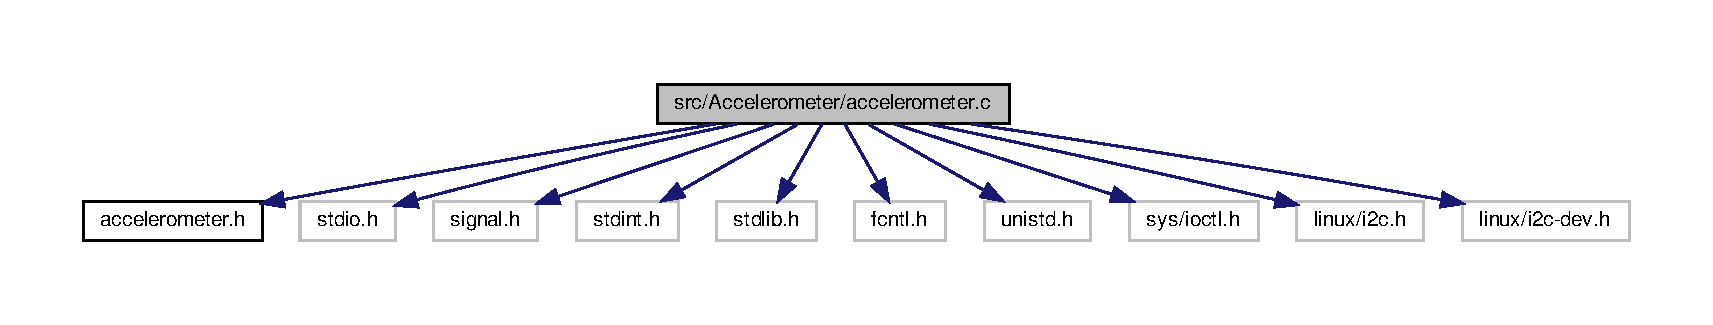
\includegraphics[width=350pt]{accelerometer_8c__incl}
\end{center}
\end{figure}
\subsection*{Functions}
\begin{DoxyCompactItemize}
\item 
void \hyperlink{accelerometer_8c_a7c5f144d9a53b740d4241be5ecf700f1}{acc\+\_\+write\+\_\+register} (uint8\+\_\+t reg, uint8\+\_\+t data)
\item 
void \hyperlink{accelerometer_8c_ae257b8efacf1001cf37944ebf81582b2}{acc\+\_\+read} (\hyperlink{structacc__t}{acc\+\_\+t} $\ast$acc)
\begin{DoxyCompactList}\small\item\em Read last acceleration measurement from device. \end{DoxyCompactList}\item 
void \hyperlink{accelerometer_8c_a4738b3c11245be7180336375f685206f}{acc\+\_\+init} ()
\begin{DoxyCompactList}\small\item\em Reset registers, disable Gyroscope and Temperature Sensor and set readings at 1.\+25 Hz. \end{DoxyCompactList}\item 
void \hyperlink{accelerometer_8c_a484dade8351c6bfb9f880a9af9890853}{acc\+\_\+close} ()
\begin{DoxyCompactList}\small\item\em Close accelerometer connection. \end{DoxyCompactList}\end{DoxyCompactItemize}


\subsection{Function Documentation}
\mbox{\Hypertarget{accelerometer_8c_a484dade8351c6bfb9f880a9af9890853}\label{accelerometer_8c_a484dade8351c6bfb9f880a9af9890853}} 
\index{accelerometer.\+c@{accelerometer.\+c}!acc\+\_\+close@{acc\+\_\+close}}
\index{acc\+\_\+close@{acc\+\_\+close}!accelerometer.\+c@{accelerometer.\+c}}
\subsubsection{\texorpdfstring{acc\+\_\+close()}{acc\_close()}}
{\footnotesize\ttfamily void acc\+\_\+close (\begin{DoxyParamCaption}{ }\end{DoxyParamCaption})}



Close accelerometer connection. 

\mbox{\Hypertarget{accelerometer_8c_a4738b3c11245be7180336375f685206f}\label{accelerometer_8c_a4738b3c11245be7180336375f685206f}} 
\index{accelerometer.\+c@{accelerometer.\+c}!acc\+\_\+init@{acc\+\_\+init}}
\index{acc\+\_\+init@{acc\+\_\+init}!accelerometer.\+c@{accelerometer.\+c}}
\subsubsection{\texorpdfstring{acc\+\_\+init()}{acc\_init()}}
{\footnotesize\ttfamily void acc\+\_\+init (\begin{DoxyParamCaption}{ }\end{DoxyParamCaption})}



Reset registers, disable Gyroscope and Temperature Sensor and set readings at 1.\+25 Hz. 

\mbox{\Hypertarget{accelerometer_8c_ae257b8efacf1001cf37944ebf81582b2}\label{accelerometer_8c_ae257b8efacf1001cf37944ebf81582b2}} 
\index{accelerometer.\+c@{accelerometer.\+c}!acc\+\_\+read@{acc\+\_\+read}}
\index{acc\+\_\+read@{acc\+\_\+read}!accelerometer.\+c@{accelerometer.\+c}}
\subsubsection{\texorpdfstring{acc\+\_\+read()}{acc\_read()}}
{\footnotesize\ttfamily void acc\+\_\+read (\begin{DoxyParamCaption}\item[{\hyperlink{structacc__t}{acc\+\_\+t} $\ast$}]{acc }\end{DoxyParamCaption})}



Read last acceleration measurement from device. 


\begin{DoxyParams}{Parameters}
{\em acc} & Pointer to the struct to save the data \\
\hline
\end{DoxyParams}
\mbox{\Hypertarget{accelerometer_8c_a7c5f144d9a53b740d4241be5ecf700f1}\label{accelerometer_8c_a7c5f144d9a53b740d4241be5ecf700f1}} 
\index{accelerometer.\+c@{accelerometer.\+c}!acc\+\_\+write\+\_\+register@{acc\+\_\+write\+\_\+register}}
\index{acc\+\_\+write\+\_\+register@{acc\+\_\+write\+\_\+register}!accelerometer.\+c@{accelerometer.\+c}}
\subsubsection{\texorpdfstring{acc\+\_\+write\+\_\+register()}{acc\_write\_register()}}
{\footnotesize\ttfamily void acc\+\_\+write\+\_\+register (\begin{DoxyParamCaption}\item[{uint8\+\_\+t}]{reg,  }\item[{uint8\+\_\+t}]{data }\end{DoxyParamCaption})}


\hypertarget{accelerometer_8h}{}\section{src/\+Accelerometer/accelerometer.h File Reference}
\label{accelerometer_8h}\index{src/\+Accelerometer/accelerometer.\+h@{src/\+Accelerometer/accelerometer.\+h}}
This graph shows which files directly or indirectly include this file\+:
\nopagebreak
\begin{figure}[H]
\begin{center}
\leavevmode
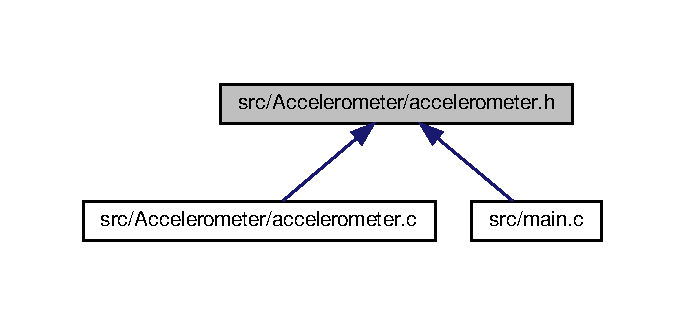
\includegraphics[width=329pt]{accelerometer_8h__dep__incl}
\end{center}
\end{figure}
\subsection*{Classes}
\begin{DoxyCompactItemize}
\item 
struct \hyperlink{structacc__t}{acc\+\_\+t}
\begin{DoxyCompactList}\small\item\em Structure to store the acceleration values as doubles. \end{DoxyCompactList}\end{DoxyCompactItemize}
\subsection*{Macros}
\begin{DoxyCompactItemize}
\item 
\#define \hyperlink{accelerometer_8h_a18d84c81f16340967647972c0d6eb452}{A\+C\+C\+\_\+\+I2\+C\+\_\+\+D\+E\+V\+I\+CE}~\char`\"{}/dev/i2c-\/1\char`\"{}
\item 
\#define \hyperlink{accelerometer_8h_a9f124818f524841838a7537856f07cdb}{A\+C\+C\+\_\+\+I2\+C\+\_\+\+S\+L\+A\+V\+E\+\_\+\+A\+D\+D\+R\+E\+SS}~0x68
\item 
\#define \hyperlink{accelerometer_8h_a604d4495d7e2d97a08991a5bd9584efb}{A\+C\+C\+\_\+\+R\+E\+G\+\_\+\+B\+A\+SE}~0x3B
\item 
\#define \hyperlink{accelerometer_8h_a1a945d17b24e537d12d2401da4233cc5}{A\+C\+C\+\_\+\+P\+O\+W\+E\+R\+\_\+\+R\+E\+G\+\_\+1}~0x6B
\item 
\#define \hyperlink{accelerometer_8h_af291eeb7d6508cb7437987e44a401d69}{A\+C\+C\+\_\+\+P\+O\+W\+E\+R\+\_\+\+R\+E\+G\+\_\+2}~0x6C
\end{DoxyCompactItemize}
\subsection*{Functions}
\begin{DoxyCompactItemize}
\item 
void \hyperlink{accelerometer_8h_a4738b3c11245be7180336375f685206f}{acc\+\_\+init} ()
\begin{DoxyCompactList}\small\item\em Reset registers, disable Gyroscope and Temperature Sensor and set readings at 1.\+25 Hz. \end{DoxyCompactList}\item 
void \hyperlink{accelerometer_8h_ae257b8efacf1001cf37944ebf81582b2}{acc\+\_\+read} (\hyperlink{structacc__t}{acc\+\_\+t} $\ast$acc)
\begin{DoxyCompactList}\small\item\em Read last acceleration measurement from device. \end{DoxyCompactList}\item 
void \hyperlink{accelerometer_8h_a484dade8351c6bfb9f880a9af9890853}{acc\+\_\+close} ()
\begin{DoxyCompactList}\small\item\em Close accelerometer connection. \end{DoxyCompactList}\end{DoxyCompactItemize}


\subsection{Macro Definition Documentation}
\mbox{\Hypertarget{accelerometer_8h_a18d84c81f16340967647972c0d6eb452}\label{accelerometer_8h_a18d84c81f16340967647972c0d6eb452}} 
\index{accelerometer.\+h@{accelerometer.\+h}!A\+C\+C\+\_\+\+I2\+C\+\_\+\+D\+E\+V\+I\+CE@{A\+C\+C\+\_\+\+I2\+C\+\_\+\+D\+E\+V\+I\+CE}}
\index{A\+C\+C\+\_\+\+I2\+C\+\_\+\+D\+E\+V\+I\+CE@{A\+C\+C\+\_\+\+I2\+C\+\_\+\+D\+E\+V\+I\+CE}!accelerometer.\+h@{accelerometer.\+h}}
\subsubsection{\texorpdfstring{A\+C\+C\+\_\+\+I2\+C\+\_\+\+D\+E\+V\+I\+CE}{ACC\_I2C\_DEVICE}}
{\footnotesize\ttfamily \#define A\+C\+C\+\_\+\+I2\+C\+\_\+\+D\+E\+V\+I\+CE~\char`\"{}/dev/i2c-\/1\char`\"{}}

\mbox{\Hypertarget{accelerometer_8h_a9f124818f524841838a7537856f07cdb}\label{accelerometer_8h_a9f124818f524841838a7537856f07cdb}} 
\index{accelerometer.\+h@{accelerometer.\+h}!A\+C\+C\+\_\+\+I2\+C\+\_\+\+S\+L\+A\+V\+E\+\_\+\+A\+D\+D\+R\+E\+SS@{A\+C\+C\+\_\+\+I2\+C\+\_\+\+S\+L\+A\+V\+E\+\_\+\+A\+D\+D\+R\+E\+SS}}
\index{A\+C\+C\+\_\+\+I2\+C\+\_\+\+S\+L\+A\+V\+E\+\_\+\+A\+D\+D\+R\+E\+SS@{A\+C\+C\+\_\+\+I2\+C\+\_\+\+S\+L\+A\+V\+E\+\_\+\+A\+D\+D\+R\+E\+SS}!accelerometer.\+h@{accelerometer.\+h}}
\subsubsection{\texorpdfstring{A\+C\+C\+\_\+\+I2\+C\+\_\+\+S\+L\+A\+V\+E\+\_\+\+A\+D\+D\+R\+E\+SS}{ACC\_I2C\_SLAVE\_ADDRESS}}
{\footnotesize\ttfamily \#define A\+C\+C\+\_\+\+I2\+C\+\_\+\+S\+L\+A\+V\+E\+\_\+\+A\+D\+D\+R\+E\+SS~0x68}

\mbox{\Hypertarget{accelerometer_8h_a1a945d17b24e537d12d2401da4233cc5}\label{accelerometer_8h_a1a945d17b24e537d12d2401da4233cc5}} 
\index{accelerometer.\+h@{accelerometer.\+h}!A\+C\+C\+\_\+\+P\+O\+W\+E\+R\+\_\+\+R\+E\+G\+\_\+1@{A\+C\+C\+\_\+\+P\+O\+W\+E\+R\+\_\+\+R\+E\+G\+\_\+1}}
\index{A\+C\+C\+\_\+\+P\+O\+W\+E\+R\+\_\+\+R\+E\+G\+\_\+1@{A\+C\+C\+\_\+\+P\+O\+W\+E\+R\+\_\+\+R\+E\+G\+\_\+1}!accelerometer.\+h@{accelerometer.\+h}}
\subsubsection{\texorpdfstring{A\+C\+C\+\_\+\+P\+O\+W\+E\+R\+\_\+\+R\+E\+G\+\_\+1}{ACC\_POWER\_REG\_1}}
{\footnotesize\ttfamily \#define A\+C\+C\+\_\+\+P\+O\+W\+E\+R\+\_\+\+R\+E\+G\+\_\+1~0x6B}

\mbox{\Hypertarget{accelerometer_8h_af291eeb7d6508cb7437987e44a401d69}\label{accelerometer_8h_af291eeb7d6508cb7437987e44a401d69}} 
\index{accelerometer.\+h@{accelerometer.\+h}!A\+C\+C\+\_\+\+P\+O\+W\+E\+R\+\_\+\+R\+E\+G\+\_\+2@{A\+C\+C\+\_\+\+P\+O\+W\+E\+R\+\_\+\+R\+E\+G\+\_\+2}}
\index{A\+C\+C\+\_\+\+P\+O\+W\+E\+R\+\_\+\+R\+E\+G\+\_\+2@{A\+C\+C\+\_\+\+P\+O\+W\+E\+R\+\_\+\+R\+E\+G\+\_\+2}!accelerometer.\+h@{accelerometer.\+h}}
\subsubsection{\texorpdfstring{A\+C\+C\+\_\+\+P\+O\+W\+E\+R\+\_\+\+R\+E\+G\+\_\+2}{ACC\_POWER\_REG\_2}}
{\footnotesize\ttfamily \#define A\+C\+C\+\_\+\+P\+O\+W\+E\+R\+\_\+\+R\+E\+G\+\_\+2~0x6C}

\mbox{\Hypertarget{accelerometer_8h_a604d4495d7e2d97a08991a5bd9584efb}\label{accelerometer_8h_a604d4495d7e2d97a08991a5bd9584efb}} 
\index{accelerometer.\+h@{accelerometer.\+h}!A\+C\+C\+\_\+\+R\+E\+G\+\_\+\+B\+A\+SE@{A\+C\+C\+\_\+\+R\+E\+G\+\_\+\+B\+A\+SE}}
\index{A\+C\+C\+\_\+\+R\+E\+G\+\_\+\+B\+A\+SE@{A\+C\+C\+\_\+\+R\+E\+G\+\_\+\+B\+A\+SE}!accelerometer.\+h@{accelerometer.\+h}}
\subsubsection{\texorpdfstring{A\+C\+C\+\_\+\+R\+E\+G\+\_\+\+B\+A\+SE}{ACC\_REG\_BASE}}
{\footnotesize\ttfamily \#define A\+C\+C\+\_\+\+R\+E\+G\+\_\+\+B\+A\+SE~0x3B}



\subsection{Function Documentation}
\mbox{\Hypertarget{accelerometer_8h_a484dade8351c6bfb9f880a9af9890853}\label{accelerometer_8h_a484dade8351c6bfb9f880a9af9890853}} 
\index{accelerometer.\+h@{accelerometer.\+h}!acc\+\_\+close@{acc\+\_\+close}}
\index{acc\+\_\+close@{acc\+\_\+close}!accelerometer.\+h@{accelerometer.\+h}}
\subsubsection{\texorpdfstring{acc\+\_\+close()}{acc\_close()}}
{\footnotesize\ttfamily void acc\+\_\+close (\begin{DoxyParamCaption}{ }\end{DoxyParamCaption})}



Close accelerometer connection. 

\mbox{\Hypertarget{accelerometer_8h_a4738b3c11245be7180336375f685206f}\label{accelerometer_8h_a4738b3c11245be7180336375f685206f}} 
\index{accelerometer.\+h@{accelerometer.\+h}!acc\+\_\+init@{acc\+\_\+init}}
\index{acc\+\_\+init@{acc\+\_\+init}!accelerometer.\+h@{accelerometer.\+h}}
\subsubsection{\texorpdfstring{acc\+\_\+init()}{acc\_init()}}
{\footnotesize\ttfamily void acc\+\_\+init (\begin{DoxyParamCaption}{ }\end{DoxyParamCaption})}



Reset registers, disable Gyroscope and Temperature Sensor and set readings at 1.\+25 Hz. 

\mbox{\Hypertarget{accelerometer_8h_ae257b8efacf1001cf37944ebf81582b2}\label{accelerometer_8h_ae257b8efacf1001cf37944ebf81582b2}} 
\index{accelerometer.\+h@{accelerometer.\+h}!acc\+\_\+read@{acc\+\_\+read}}
\index{acc\+\_\+read@{acc\+\_\+read}!accelerometer.\+h@{accelerometer.\+h}}
\subsubsection{\texorpdfstring{acc\+\_\+read()}{acc\_read()}}
{\footnotesize\ttfamily void acc\+\_\+read (\begin{DoxyParamCaption}\item[{\hyperlink{structacc__t}{acc\+\_\+t} $\ast$}]{acc }\end{DoxyParamCaption})}



Read last acceleration measurement from device. 


\begin{DoxyParams}{Parameters}
{\em acc} & Pointer to the struct to save the data \\
\hline
\end{DoxyParams}

\hypertarget{colorSensor_8c}{}\section{src/\+Color\+Sensor/color\+Sensor.c File Reference}
\label{colorSensor_8c}\index{src/\+Color\+Sensor/color\+Sensor.\+c@{src/\+Color\+Sensor/color\+Sensor.\+c}}
{\ttfamily \#include \char`\"{}color\+Sensor.\+h\char`\"{}}\newline
{\ttfamily \#include $<$stdio.\+h$>$}\newline
{\ttfamily \#include $<$signal.\+h$>$}\newline
{\ttfamily \#include $<$stdint.\+h$>$}\newline
{\ttfamily \#include $<$stdlib.\+h$>$}\newline
{\ttfamily \#include $<$fcntl.\+h$>$}\newline
{\ttfamily \#include $<$unistd.\+h$>$}\newline
{\ttfamily \#include $<$sys/ioctl.\+h$>$}\newline
{\ttfamily \#include $<$linux/i2c.\+h$>$}\newline
{\ttfamily \#include $<$linux/i2c-\/dev.\+h$>$}\newline
Include dependency graph for color\+Sensor.\+c\+:\nopagebreak
\begin{figure}[H]
\begin{center}
\leavevmode
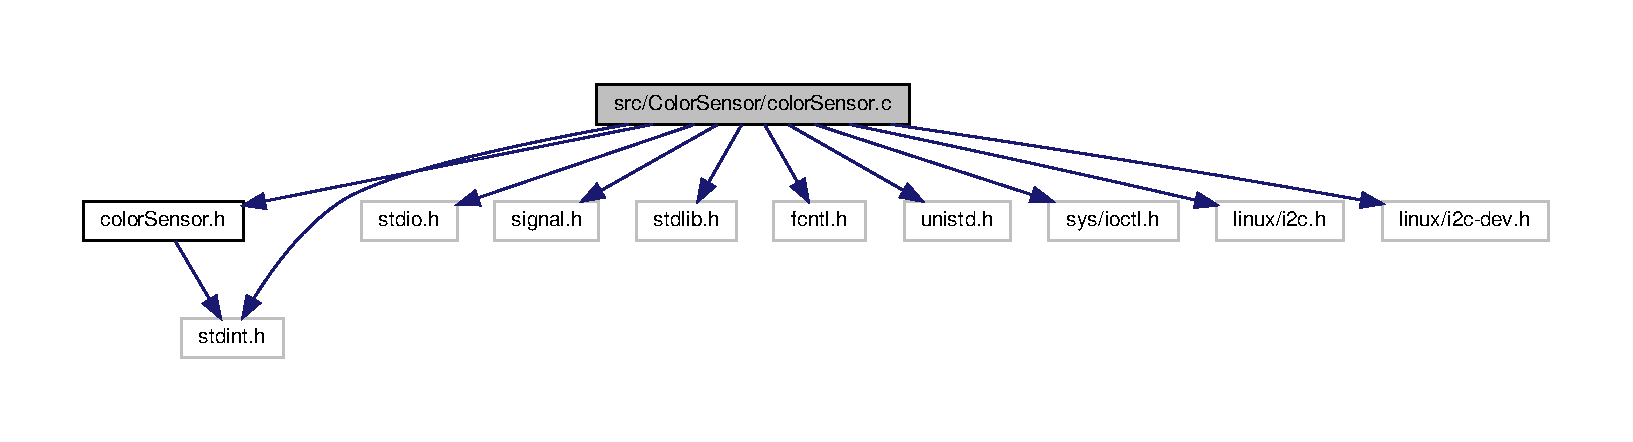
\includegraphics[width=350pt]{colorSensor_8c__incl}
\end{center}
\end{figure}
\subsection*{Macros}
\begin{DoxyCompactItemize}
\item 
\#define \hyperlink{colorSensor_8c_ad2f3678bf5eae3684fc497130b946eae}{M\+IN}(X,  Y)~(((X) $<$ (Y)) ? (X) \+: (Y))
\item 
\#define \hyperlink{colorSensor_8c_aff9931d7524c88e07743af6535b20761}{M\+AX}(X,  Y)~(((X) $>$ (Y)) ? (X) \+: (Y))
\end{DoxyCompactItemize}
\subsection*{Functions}
\begin{DoxyCompactItemize}
\item 
void \hyperlink{colorSensor_8c_a54172ee220319e4c3eb259338946405b}{cs\+\_\+write\+\_\+register} (uint8\+\_\+t reg, uint8\+\_\+t data)
\item 
void \hyperlink{colorSensor_8c_a98d00cbfc6cb3d3c72b859da7b824628}{cs\+\_\+init} ()
\begin{DoxyCompactList}\small\item\em Initializes the color sensor in periodic read mode. \end{DoxyCompactList}\item 
void \hyperlink{colorSensor_8c_a8a960d450999b5c49697c155c3364fbb}{cs\+\_\+close} ()
\begin{DoxyCompactList}\small\item\em Controlledly closes the sensor object. \end{DoxyCompactList}\item 
int \hyperlink{colorSensor_8c_ae07874642d6dc0f27eb1521ecbfae1dc}{cs\+\_\+read\+\_\+clear\+\_\+corrected} (\hyperlink{structcolor__t}{color\+\_\+t} $\ast$color)
\begin{DoxyCompactList}\small\item\em Read the color and clear correct it. \end{DoxyCompactList}\item 
int \hyperlink{colorSensor_8c_a747039a0f6945a4f6fd9ee7102bbff36}{cs\+\_\+read\+\_\+raw} (\hyperlink{structcolor__t}{color\+\_\+t} $\ast$color)
\begin{DoxyCompactList}\small\item\em Read the color raw. \end{DoxyCompactList}\end{DoxyCompactItemize}


\subsection{Macro Definition Documentation}
\mbox{\Hypertarget{colorSensor_8c_aff9931d7524c88e07743af6535b20761}\label{colorSensor_8c_aff9931d7524c88e07743af6535b20761}} 
\index{color\+Sensor.\+c@{color\+Sensor.\+c}!M\+AX@{M\+AX}}
\index{M\+AX@{M\+AX}!color\+Sensor.\+c@{color\+Sensor.\+c}}
\subsubsection{\texorpdfstring{M\+AX}{MAX}}
{\footnotesize\ttfamily \#define M\+AX(\begin{DoxyParamCaption}\item[{}]{X,  }\item[{}]{Y }\end{DoxyParamCaption})~(((X) $>$ (Y)) ? (X) \+: (Y))}

\mbox{\Hypertarget{colorSensor_8c_ad2f3678bf5eae3684fc497130b946eae}\label{colorSensor_8c_ad2f3678bf5eae3684fc497130b946eae}} 
\index{color\+Sensor.\+c@{color\+Sensor.\+c}!M\+IN@{M\+IN}}
\index{M\+IN@{M\+IN}!color\+Sensor.\+c@{color\+Sensor.\+c}}
\subsubsection{\texorpdfstring{M\+IN}{MIN}}
{\footnotesize\ttfamily \#define M\+IN(\begin{DoxyParamCaption}\item[{}]{X,  }\item[{}]{Y }\end{DoxyParamCaption})~(((X) $<$ (Y)) ? (X) \+: (Y))}



\subsection{Function Documentation}
\mbox{\Hypertarget{colorSensor_8c_a8a960d450999b5c49697c155c3364fbb}\label{colorSensor_8c_a8a960d450999b5c49697c155c3364fbb}} 
\index{color\+Sensor.\+c@{color\+Sensor.\+c}!cs\+\_\+close@{cs\+\_\+close}}
\index{cs\+\_\+close@{cs\+\_\+close}!color\+Sensor.\+c@{color\+Sensor.\+c}}
\subsubsection{\texorpdfstring{cs\+\_\+close()}{cs\_close()}}
{\footnotesize\ttfamily void cs\+\_\+close (\begin{DoxyParamCaption}{ }\end{DoxyParamCaption})}



Controlledly closes the sensor object. 

\mbox{\Hypertarget{colorSensor_8c_a98d00cbfc6cb3d3c72b859da7b824628}\label{colorSensor_8c_a98d00cbfc6cb3d3c72b859da7b824628}} 
\index{color\+Sensor.\+c@{color\+Sensor.\+c}!cs\+\_\+init@{cs\+\_\+init}}
\index{cs\+\_\+init@{cs\+\_\+init}!color\+Sensor.\+c@{color\+Sensor.\+c}}
\subsubsection{\texorpdfstring{cs\+\_\+init()}{cs\_init()}}
{\footnotesize\ttfamily void cs\+\_\+init (\begin{DoxyParamCaption}{ }\end{DoxyParamCaption})}



Initializes the color sensor in periodic read mode. 

\mbox{\Hypertarget{colorSensor_8c_ae07874642d6dc0f27eb1521ecbfae1dc}\label{colorSensor_8c_ae07874642d6dc0f27eb1521ecbfae1dc}} 
\index{color\+Sensor.\+c@{color\+Sensor.\+c}!cs\+\_\+read\+\_\+clear\+\_\+corrected@{cs\+\_\+read\+\_\+clear\+\_\+corrected}}
\index{cs\+\_\+read\+\_\+clear\+\_\+corrected@{cs\+\_\+read\+\_\+clear\+\_\+corrected}!color\+Sensor.\+c@{color\+Sensor.\+c}}
\subsubsection{\texorpdfstring{cs\+\_\+read\+\_\+clear\+\_\+corrected()}{cs\_read\_clear\_corrected()}}
{\footnotesize\ttfamily int cs\+\_\+read\+\_\+clear\+\_\+corrected (\begin{DoxyParamCaption}\item[{\hyperlink{structcolor__t}{color\+\_\+t} $\ast$}]{color }\end{DoxyParamCaption})}



Read the color and clear correct it. 


\begin{DoxyParams}{Parameters}
{\em color} & Pointer to the structure to store the color information \\
\hline
\end{DoxyParams}
\begin{DoxyReturn}{Returns}
(int) Exit code of the operation 
\end{DoxyReturn}
\mbox{\Hypertarget{colorSensor_8c_a747039a0f6945a4f6fd9ee7102bbff36}\label{colorSensor_8c_a747039a0f6945a4f6fd9ee7102bbff36}} 
\index{color\+Sensor.\+c@{color\+Sensor.\+c}!cs\+\_\+read\+\_\+raw@{cs\+\_\+read\+\_\+raw}}
\index{cs\+\_\+read\+\_\+raw@{cs\+\_\+read\+\_\+raw}!color\+Sensor.\+c@{color\+Sensor.\+c}}
\subsubsection{\texorpdfstring{cs\+\_\+read\+\_\+raw()}{cs\_read\_raw()}}
{\footnotesize\ttfamily int cs\+\_\+read\+\_\+raw (\begin{DoxyParamCaption}\item[{\hyperlink{structcolor__t}{color\+\_\+t} $\ast$}]{color }\end{DoxyParamCaption})}



Read the color raw. 


\begin{DoxyParams}{Parameters}
{\em color} & Pointer to the structure to store the color information \\
\hline
\end{DoxyParams}
\begin{DoxyReturn}{Returns}
(int) Exit code of the operation 
\end{DoxyReturn}
\mbox{\Hypertarget{colorSensor_8c_a54172ee220319e4c3eb259338946405b}\label{colorSensor_8c_a54172ee220319e4c3eb259338946405b}} 
\index{color\+Sensor.\+c@{color\+Sensor.\+c}!cs\+\_\+write\+\_\+register@{cs\+\_\+write\+\_\+register}}
\index{cs\+\_\+write\+\_\+register@{cs\+\_\+write\+\_\+register}!color\+Sensor.\+c@{color\+Sensor.\+c}}
\subsubsection{\texorpdfstring{cs\+\_\+write\+\_\+register()}{cs\_write\_register()}}
{\footnotesize\ttfamily void cs\+\_\+write\+\_\+register (\begin{DoxyParamCaption}\item[{uint8\+\_\+t}]{reg,  }\item[{uint8\+\_\+t}]{data }\end{DoxyParamCaption})}


\hypertarget{colorSensor_8h}{}\section{src/\+Color\+Sensor/color\+Sensor.h File Reference}
\label{colorSensor_8h}\index{src/\+Color\+Sensor/color\+Sensor.\+h@{src/\+Color\+Sensor/color\+Sensor.\+h}}
{\ttfamily \#include $<$stdint.\+h$>$}\newline
Include dependency graph for color\+Sensor.\+h\+:
\nopagebreak
\begin{figure}[H]
\begin{center}
\leavevmode
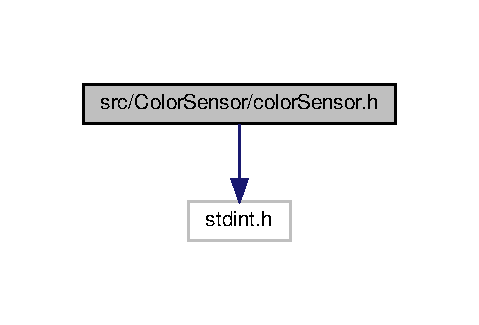
\includegraphics[width=230pt]{colorSensor_8h__incl}
\end{center}
\end{figure}
This graph shows which files directly or indirectly include this file\+:
\nopagebreak
\begin{figure}[H]
\begin{center}
\leavevmode
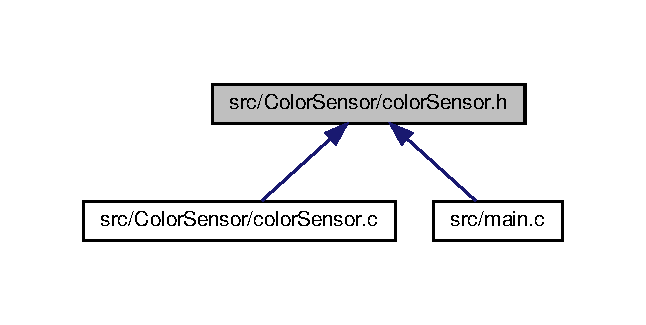
\includegraphics[width=310pt]{colorSensor_8h__dep__incl}
\end{center}
\end{figure}
\subsection*{Classes}
\begin{DoxyCompactItemize}
\item 
struct \hyperlink{structrgb__color__t}{rgb\+\_\+color\+\_\+t}
\begin{DoxyCompactList}\small\item\em Basic struct for an R\+GB color. Contains the three colors as unsigned 8 bits. \end{DoxyCompactList}\item 
struct \hyperlink{structcomplete__color__t}{complete\+\_\+color\+\_\+t}
\begin{DoxyCompactList}\small\item\em Advanced color structure. Contains the rgbc color, the corrected rgb, the IR, temperature, saturation and lux values. \end{DoxyCompactList}\end{DoxyCompactItemize}
\subsection*{Macros}
\begin{DoxyCompactItemize}
\item 
\#define \hyperlink{colorSensor_8h_a7ac144fbb22a44749e5071fc8a3768f8}{C\+O\+L\+O\+R\+\_\+\+S\+E\+N\+S\+O\+R\+\_\+\+S\+L\+A\+V\+E\+\_\+\+A\+D\+D\+R\+E\+SS}~0x29
\item 
\#define \hyperlink{colorSensor_8h_a29054016a6feea652c2cc21dc8675a7e}{C\+O\+L\+O\+R\+\_\+\+S\+E\+N\+S\+O\+R\+\_\+\+I2\+C\+\_\+\+D\+E\+V\+I\+CE}~\char`\"{}/dev/i2c-\/1\char`\"{}
\item 
\#define \hyperlink{colorSensor_8h_a2c1a60a3b3c45782008d0b48d35dc2d8}{C\+O\+L\+O\+R\+\_\+\+S\+E\+N\+S\+O\+R\+\_\+\+C\+O\+M\+M\+A\+ND}~0x80
\item 
\#define \hyperlink{colorSensor_8h_ab53e2cd3502c808ce7a99285bac868cc}{C\+O\+L\+O\+R\+\_\+\+S\+E\+N\+S\+O\+R\+\_\+\+O\+N\+CE}~0x00
\item 
\#define \hyperlink{colorSensor_8h_a6ade3980ade53e90e688916212688281}{C\+O\+L\+O\+R\+\_\+\+S\+E\+N\+S\+O\+R\+\_\+\+I\+NC}~0x20
\item 
\#define \hyperlink{colorSensor_8h_a1599c80be0f8318e5bb8b1ba69c076f7}{C\+O\+L\+O\+R\+\_\+\+S\+E\+N\+S\+O\+R\+\_\+\+E\+N\+A\+B\+LE}~0x00
\item 
\#define \hyperlink{colorSensor_8h_a90e4e314713e5453fc71b31788f7f6dc}{C\+O\+L\+O\+R\+\_\+\+S\+E\+N\+S\+O\+R\+\_\+\+A\+T\+I\+ME}~0x01
\item 
\#define \hyperlink{colorSensor_8h_a6d186b50af4561378508a4f594e3bb9a}{C\+O\+L\+O\+R\+\_\+\+S\+E\+N\+S\+O\+R\+\_\+\+W\+T\+I\+ME}~0x03
\item 
\#define \hyperlink{colorSensor_8h_a521a5943cbeff2436d97a825f73ff735}{C\+O\+L\+O\+R\+\_\+\+S\+E\+N\+S\+O\+R\+\_\+\+A\+I\+L\+TL}~0x04
\item 
\#define \hyperlink{colorSensor_8h_ab66be2c885b3b30f8817f8b40db05717}{C\+O\+L\+O\+R\+\_\+\+S\+E\+N\+S\+O\+R\+\_\+\+A\+I\+L\+TH}~0x05
\item 
\#define \hyperlink{colorSensor_8h_a8b3c59f95f915b7910d95d12d6c98294}{C\+O\+L\+O\+R\+\_\+\+S\+E\+N\+S\+O\+R\+\_\+\+A\+I\+H\+TL}~0x06
\item 
\#define \hyperlink{colorSensor_8h_ade5ab6415b0ae40c662929cd8fcc988e}{C\+O\+L\+O\+R\+\_\+\+S\+E\+N\+S\+O\+R\+\_\+\+A\+I\+H\+TH}~0x07
\item 
\#define \hyperlink{colorSensor_8h_a9b7348d15e45d2d84c2dbc9963937b45}{C\+O\+L\+O\+R\+\_\+\+S\+E\+N\+S\+O\+R\+\_\+\+P\+E\+RS}~0x0C
\item 
\#define \hyperlink{colorSensor_8h_a9b95e1556fcb8168884472b8d4fa0837}{C\+O\+L\+O\+R\+\_\+\+S\+E\+N\+S\+O\+R\+\_\+\+C\+O\+N\+F\+IG}~0x0D
\item 
\#define \hyperlink{colorSensor_8h_af7d946bb0f306d5d6e44391a4381ccc6}{C\+O\+L\+O\+R\+\_\+\+S\+E\+N\+S\+O\+R\+\_\+\+C\+O\+N\+T\+R\+OL}~0x0F
\item 
\#define \hyperlink{colorSensor_8h_a73773e44f564733a8707bba6387f0499}{C\+O\+L\+O\+R\+\_\+\+S\+E\+N\+S\+O\+R\+\_\+\+ID}~0x12
\item 
\#define \hyperlink{colorSensor_8h_a72ea5a22b44e896033c44c96f5852f88}{C\+O\+L\+O\+R\+\_\+\+S\+E\+N\+S\+O\+R\+\_\+\+S\+T\+A\+T\+US}~0x13
\item 
\#define \hyperlink{colorSensor_8h_a1e243b5efc30e5e897549a0d390b4932}{C\+O\+L\+O\+R\+\_\+\+S\+E\+N\+S\+O\+R\+\_\+\+C\+D\+A\+T\+AL}~0x14
\item 
\#define \hyperlink{colorSensor_8h_a4c4df7dab414f781bf2a882fad49a8df}{C\+O\+L\+O\+R\+\_\+\+S\+E\+N\+S\+O\+R\+\_\+\+C\+D\+A\+T\+AH}~0x15
\item 
\#define \hyperlink{colorSensor_8h_a83387249482b2dbd934a1353d615e5f4}{C\+O\+L\+O\+R\+\_\+\+S\+E\+N\+S\+O\+R\+\_\+\+R\+D\+A\+T\+AL}~0x16
\item 
\#define \hyperlink{colorSensor_8h_aafdd4b0da2356087b5f56b83865c64ed}{C\+O\+L\+O\+R\+\_\+\+S\+E\+N\+S\+O\+R\+\_\+\+R\+D\+A\+T\+AH}~0x17
\item 
\#define \hyperlink{colorSensor_8h_aea8659d64c6b794277b3688aa4e17417}{C\+O\+L\+O\+R\+\_\+\+S\+E\+N\+S\+O\+R\+\_\+\+G\+D\+A\+T\+AL}~0x18
\item 
\#define \hyperlink{colorSensor_8h_aaa1ffd51b684c2634c3993faa7387dca}{C\+O\+L\+O\+R\+\_\+\+S\+E\+N\+S\+O\+R\+\_\+\+G\+D\+A\+T\+AH}~0x19
\item 
\#define \hyperlink{colorSensor_8h_a928d1baa8a5440f3defc1214d080058a}{C\+O\+L\+O\+R\+\_\+\+S\+E\+N\+S\+O\+R\+\_\+\+B\+D\+A\+T\+AL}~0x1A
\item 
\#define \hyperlink{colorSensor_8h_a6cbd1074652a01b15b440808ea5a0239}{C\+O\+L\+O\+R\+\_\+\+S\+E\+N\+S\+O\+R\+\_\+\+B\+D\+A\+T\+AH}~0x1B
\item 
\#define \hyperlink{colorSensor_8h_a788035f03e452c41055ddcfebb40d163}{C\+O\+L\+O\+R\+\_\+\+S\+E\+N\+S\+O\+R\+\_\+\+GA}~1
\item 
\#define \hyperlink{colorSensor_8h_a628ed3f112699765f0fa36f5f38c77d3}{C\+O\+L\+O\+R\+\_\+\+S\+E\+N\+S\+O\+R\+\_\+\+DF}~310
\item 
\#define \hyperlink{colorSensor_8h_a25931c3d7ab21bfbfffc55582fcd5c0f}{C\+O\+L\+O\+R\+\_\+\+S\+E\+N\+S\+O\+R\+\_\+\+R\+\_\+\+C\+O\+EF}~0.\+136f
\item 
\#define \hyperlink{colorSensor_8h_a2b02c79f60614bc41244684cf3da3fb2}{C\+O\+L\+O\+R\+\_\+\+S\+E\+N\+S\+O\+R\+\_\+\+G\+\_\+\+C\+O\+EF}~1
\item 
\#define \hyperlink{colorSensor_8h_a236fa009169ce7376bc9ad08d97a7fca}{C\+O\+L\+O\+R\+\_\+\+S\+E\+N\+S\+O\+R\+\_\+\+B\+\_\+\+C\+O\+EF}~-\/0.\+444
\item 
\#define \hyperlink{colorSensor_8h_a257ef1e4bbc289731b30cce9f8e8dbba}{C\+O\+L\+O\+R\+\_\+\+S\+E\+N\+S\+O\+R\+\_\+\+C\+T\+\_\+\+C\+O\+EF}~3810
\item 
\#define \hyperlink{colorSensor_8h_a066a9e81a879aeffcc395e5f7d59c76f}{C\+O\+L\+O\+R\+\_\+\+S\+E\+N\+S\+O\+R\+\_\+\+C\+T\+\_\+\+O\+FF}~1391
\end{DoxyCompactItemize}
\subsection*{Functions}
\begin{DoxyCompactItemize}
\item 
void \hyperlink{colorSensor_8h_a98d00cbfc6cb3d3c72b859da7b824628}{cs\+\_\+init} ()
\begin{DoxyCompactList}\small\item\em Initializes the color sensor in periodic read mode. \end{DoxyCompactList}\item 
int \hyperlink{colorSensor_8h_a77b0ffd46a52dbb4294fd7924f608de7}{cs\+\_\+read\+\_\+clear\+\_\+corrected} (\hyperlink{structrgb__color__t}{rgb\+\_\+color\+\_\+t} $\ast$color)
\begin{DoxyCompactList}\small\item\em Read the color and clear correct it. \end{DoxyCompactList}\item 
int \hyperlink{colorSensor_8h_af9d8deea040144d0382bfa8b3ca1462f}{cs\+\_\+read\+\_\+raw} (\hyperlink{structrgb__color__t}{rgb\+\_\+color\+\_\+t} $\ast$color)
\begin{DoxyCompactList}\small\item\em Read the color raw. \end{DoxyCompactList}\item 
void \hyperlink{colorSensor_8h_adf8a27fabd9c693ff2e247415945ea0e}{cs\+\_\+read\+\_\+complete} (\hyperlink{structcomplete__color__t}{complete\+\_\+color\+\_\+t} $\ast$color)
\begin{DoxyCompactList}\small\item\em Read the color and calculate all the parameters. \end{DoxyCompactList}\item 
void \hyperlink{colorSensor_8h_a8a960d450999b5c49697c155c3364fbb}{cs\+\_\+close} ()
\begin{DoxyCompactList}\small\item\em Controlledly closes the sensor object. \end{DoxyCompactList}\end{DoxyCompactItemize}


\subsection{Macro Definition Documentation}
\mbox{\Hypertarget{colorSensor_8h_ade5ab6415b0ae40c662929cd8fcc988e}\label{colorSensor_8h_ade5ab6415b0ae40c662929cd8fcc988e}} 
\index{color\+Sensor.\+h@{color\+Sensor.\+h}!C\+O\+L\+O\+R\+\_\+\+S\+E\+N\+S\+O\+R\+\_\+\+A\+I\+H\+TH@{C\+O\+L\+O\+R\+\_\+\+S\+E\+N\+S\+O\+R\+\_\+\+A\+I\+H\+TH}}
\index{C\+O\+L\+O\+R\+\_\+\+S\+E\+N\+S\+O\+R\+\_\+\+A\+I\+H\+TH@{C\+O\+L\+O\+R\+\_\+\+S\+E\+N\+S\+O\+R\+\_\+\+A\+I\+H\+TH}!color\+Sensor.\+h@{color\+Sensor.\+h}}
\subsubsection{\texorpdfstring{C\+O\+L\+O\+R\+\_\+\+S\+E\+N\+S\+O\+R\+\_\+\+A\+I\+H\+TH}{COLOR\_SENSOR\_AIHTH}}
{\footnotesize\ttfamily \#define C\+O\+L\+O\+R\+\_\+\+S\+E\+N\+S\+O\+R\+\_\+\+A\+I\+H\+TH~0x07}

\mbox{\Hypertarget{colorSensor_8h_a8b3c59f95f915b7910d95d12d6c98294}\label{colorSensor_8h_a8b3c59f95f915b7910d95d12d6c98294}} 
\index{color\+Sensor.\+h@{color\+Sensor.\+h}!C\+O\+L\+O\+R\+\_\+\+S\+E\+N\+S\+O\+R\+\_\+\+A\+I\+H\+TL@{C\+O\+L\+O\+R\+\_\+\+S\+E\+N\+S\+O\+R\+\_\+\+A\+I\+H\+TL}}
\index{C\+O\+L\+O\+R\+\_\+\+S\+E\+N\+S\+O\+R\+\_\+\+A\+I\+H\+TL@{C\+O\+L\+O\+R\+\_\+\+S\+E\+N\+S\+O\+R\+\_\+\+A\+I\+H\+TL}!color\+Sensor.\+h@{color\+Sensor.\+h}}
\subsubsection{\texorpdfstring{C\+O\+L\+O\+R\+\_\+\+S\+E\+N\+S\+O\+R\+\_\+\+A\+I\+H\+TL}{COLOR\_SENSOR\_AIHTL}}
{\footnotesize\ttfamily \#define C\+O\+L\+O\+R\+\_\+\+S\+E\+N\+S\+O\+R\+\_\+\+A\+I\+H\+TL~0x06}

\mbox{\Hypertarget{colorSensor_8h_ab66be2c885b3b30f8817f8b40db05717}\label{colorSensor_8h_ab66be2c885b3b30f8817f8b40db05717}} 
\index{color\+Sensor.\+h@{color\+Sensor.\+h}!C\+O\+L\+O\+R\+\_\+\+S\+E\+N\+S\+O\+R\+\_\+\+A\+I\+L\+TH@{C\+O\+L\+O\+R\+\_\+\+S\+E\+N\+S\+O\+R\+\_\+\+A\+I\+L\+TH}}
\index{C\+O\+L\+O\+R\+\_\+\+S\+E\+N\+S\+O\+R\+\_\+\+A\+I\+L\+TH@{C\+O\+L\+O\+R\+\_\+\+S\+E\+N\+S\+O\+R\+\_\+\+A\+I\+L\+TH}!color\+Sensor.\+h@{color\+Sensor.\+h}}
\subsubsection{\texorpdfstring{C\+O\+L\+O\+R\+\_\+\+S\+E\+N\+S\+O\+R\+\_\+\+A\+I\+L\+TH}{COLOR\_SENSOR\_AILTH}}
{\footnotesize\ttfamily \#define C\+O\+L\+O\+R\+\_\+\+S\+E\+N\+S\+O\+R\+\_\+\+A\+I\+L\+TH~0x05}

\mbox{\Hypertarget{colorSensor_8h_a521a5943cbeff2436d97a825f73ff735}\label{colorSensor_8h_a521a5943cbeff2436d97a825f73ff735}} 
\index{color\+Sensor.\+h@{color\+Sensor.\+h}!C\+O\+L\+O\+R\+\_\+\+S\+E\+N\+S\+O\+R\+\_\+\+A\+I\+L\+TL@{C\+O\+L\+O\+R\+\_\+\+S\+E\+N\+S\+O\+R\+\_\+\+A\+I\+L\+TL}}
\index{C\+O\+L\+O\+R\+\_\+\+S\+E\+N\+S\+O\+R\+\_\+\+A\+I\+L\+TL@{C\+O\+L\+O\+R\+\_\+\+S\+E\+N\+S\+O\+R\+\_\+\+A\+I\+L\+TL}!color\+Sensor.\+h@{color\+Sensor.\+h}}
\subsubsection{\texorpdfstring{C\+O\+L\+O\+R\+\_\+\+S\+E\+N\+S\+O\+R\+\_\+\+A\+I\+L\+TL}{COLOR\_SENSOR\_AILTL}}
{\footnotesize\ttfamily \#define C\+O\+L\+O\+R\+\_\+\+S\+E\+N\+S\+O\+R\+\_\+\+A\+I\+L\+TL~0x04}

\mbox{\Hypertarget{colorSensor_8h_a90e4e314713e5453fc71b31788f7f6dc}\label{colorSensor_8h_a90e4e314713e5453fc71b31788f7f6dc}} 
\index{color\+Sensor.\+h@{color\+Sensor.\+h}!C\+O\+L\+O\+R\+\_\+\+S\+E\+N\+S\+O\+R\+\_\+\+A\+T\+I\+ME@{C\+O\+L\+O\+R\+\_\+\+S\+E\+N\+S\+O\+R\+\_\+\+A\+T\+I\+ME}}
\index{C\+O\+L\+O\+R\+\_\+\+S\+E\+N\+S\+O\+R\+\_\+\+A\+T\+I\+ME@{C\+O\+L\+O\+R\+\_\+\+S\+E\+N\+S\+O\+R\+\_\+\+A\+T\+I\+ME}!color\+Sensor.\+h@{color\+Sensor.\+h}}
\subsubsection{\texorpdfstring{C\+O\+L\+O\+R\+\_\+\+S\+E\+N\+S\+O\+R\+\_\+\+A\+T\+I\+ME}{COLOR\_SENSOR\_ATIME}}
{\footnotesize\ttfamily \#define C\+O\+L\+O\+R\+\_\+\+S\+E\+N\+S\+O\+R\+\_\+\+A\+T\+I\+ME~0x01}

\mbox{\Hypertarget{colorSensor_8h_a236fa009169ce7376bc9ad08d97a7fca}\label{colorSensor_8h_a236fa009169ce7376bc9ad08d97a7fca}} 
\index{color\+Sensor.\+h@{color\+Sensor.\+h}!C\+O\+L\+O\+R\+\_\+\+S\+E\+N\+S\+O\+R\+\_\+\+B\+\_\+\+C\+O\+EF@{C\+O\+L\+O\+R\+\_\+\+S\+E\+N\+S\+O\+R\+\_\+\+B\+\_\+\+C\+O\+EF}}
\index{C\+O\+L\+O\+R\+\_\+\+S\+E\+N\+S\+O\+R\+\_\+\+B\+\_\+\+C\+O\+EF@{C\+O\+L\+O\+R\+\_\+\+S\+E\+N\+S\+O\+R\+\_\+\+B\+\_\+\+C\+O\+EF}!color\+Sensor.\+h@{color\+Sensor.\+h}}
\subsubsection{\texorpdfstring{C\+O\+L\+O\+R\+\_\+\+S\+E\+N\+S\+O\+R\+\_\+\+B\+\_\+\+C\+O\+EF}{COLOR\_SENSOR\_B\_COEF}}
{\footnotesize\ttfamily \#define C\+O\+L\+O\+R\+\_\+\+S\+E\+N\+S\+O\+R\+\_\+\+B\+\_\+\+C\+O\+EF~-\/0.\+444}

\mbox{\Hypertarget{colorSensor_8h_a6cbd1074652a01b15b440808ea5a0239}\label{colorSensor_8h_a6cbd1074652a01b15b440808ea5a0239}} 
\index{color\+Sensor.\+h@{color\+Sensor.\+h}!C\+O\+L\+O\+R\+\_\+\+S\+E\+N\+S\+O\+R\+\_\+\+B\+D\+A\+T\+AH@{C\+O\+L\+O\+R\+\_\+\+S\+E\+N\+S\+O\+R\+\_\+\+B\+D\+A\+T\+AH}}
\index{C\+O\+L\+O\+R\+\_\+\+S\+E\+N\+S\+O\+R\+\_\+\+B\+D\+A\+T\+AH@{C\+O\+L\+O\+R\+\_\+\+S\+E\+N\+S\+O\+R\+\_\+\+B\+D\+A\+T\+AH}!color\+Sensor.\+h@{color\+Sensor.\+h}}
\subsubsection{\texorpdfstring{C\+O\+L\+O\+R\+\_\+\+S\+E\+N\+S\+O\+R\+\_\+\+B\+D\+A\+T\+AH}{COLOR\_SENSOR\_BDATAH}}
{\footnotesize\ttfamily \#define C\+O\+L\+O\+R\+\_\+\+S\+E\+N\+S\+O\+R\+\_\+\+B\+D\+A\+T\+AH~0x1B}

\mbox{\Hypertarget{colorSensor_8h_a928d1baa8a5440f3defc1214d080058a}\label{colorSensor_8h_a928d1baa8a5440f3defc1214d080058a}} 
\index{color\+Sensor.\+h@{color\+Sensor.\+h}!C\+O\+L\+O\+R\+\_\+\+S\+E\+N\+S\+O\+R\+\_\+\+B\+D\+A\+T\+AL@{C\+O\+L\+O\+R\+\_\+\+S\+E\+N\+S\+O\+R\+\_\+\+B\+D\+A\+T\+AL}}
\index{C\+O\+L\+O\+R\+\_\+\+S\+E\+N\+S\+O\+R\+\_\+\+B\+D\+A\+T\+AL@{C\+O\+L\+O\+R\+\_\+\+S\+E\+N\+S\+O\+R\+\_\+\+B\+D\+A\+T\+AL}!color\+Sensor.\+h@{color\+Sensor.\+h}}
\subsubsection{\texorpdfstring{C\+O\+L\+O\+R\+\_\+\+S\+E\+N\+S\+O\+R\+\_\+\+B\+D\+A\+T\+AL}{COLOR\_SENSOR\_BDATAL}}
{\footnotesize\ttfamily \#define C\+O\+L\+O\+R\+\_\+\+S\+E\+N\+S\+O\+R\+\_\+\+B\+D\+A\+T\+AL~0x1A}

\mbox{\Hypertarget{colorSensor_8h_a4c4df7dab414f781bf2a882fad49a8df}\label{colorSensor_8h_a4c4df7dab414f781bf2a882fad49a8df}} 
\index{color\+Sensor.\+h@{color\+Sensor.\+h}!C\+O\+L\+O\+R\+\_\+\+S\+E\+N\+S\+O\+R\+\_\+\+C\+D\+A\+T\+AH@{C\+O\+L\+O\+R\+\_\+\+S\+E\+N\+S\+O\+R\+\_\+\+C\+D\+A\+T\+AH}}
\index{C\+O\+L\+O\+R\+\_\+\+S\+E\+N\+S\+O\+R\+\_\+\+C\+D\+A\+T\+AH@{C\+O\+L\+O\+R\+\_\+\+S\+E\+N\+S\+O\+R\+\_\+\+C\+D\+A\+T\+AH}!color\+Sensor.\+h@{color\+Sensor.\+h}}
\subsubsection{\texorpdfstring{C\+O\+L\+O\+R\+\_\+\+S\+E\+N\+S\+O\+R\+\_\+\+C\+D\+A\+T\+AH}{COLOR\_SENSOR\_CDATAH}}
{\footnotesize\ttfamily \#define C\+O\+L\+O\+R\+\_\+\+S\+E\+N\+S\+O\+R\+\_\+\+C\+D\+A\+T\+AH~0x15}

\mbox{\Hypertarget{colorSensor_8h_a1e243b5efc30e5e897549a0d390b4932}\label{colorSensor_8h_a1e243b5efc30e5e897549a0d390b4932}} 
\index{color\+Sensor.\+h@{color\+Sensor.\+h}!C\+O\+L\+O\+R\+\_\+\+S\+E\+N\+S\+O\+R\+\_\+\+C\+D\+A\+T\+AL@{C\+O\+L\+O\+R\+\_\+\+S\+E\+N\+S\+O\+R\+\_\+\+C\+D\+A\+T\+AL}}
\index{C\+O\+L\+O\+R\+\_\+\+S\+E\+N\+S\+O\+R\+\_\+\+C\+D\+A\+T\+AL@{C\+O\+L\+O\+R\+\_\+\+S\+E\+N\+S\+O\+R\+\_\+\+C\+D\+A\+T\+AL}!color\+Sensor.\+h@{color\+Sensor.\+h}}
\subsubsection{\texorpdfstring{C\+O\+L\+O\+R\+\_\+\+S\+E\+N\+S\+O\+R\+\_\+\+C\+D\+A\+T\+AL}{COLOR\_SENSOR\_CDATAL}}
{\footnotesize\ttfamily \#define C\+O\+L\+O\+R\+\_\+\+S\+E\+N\+S\+O\+R\+\_\+\+C\+D\+A\+T\+AL~0x14}

\mbox{\Hypertarget{colorSensor_8h_a2c1a60a3b3c45782008d0b48d35dc2d8}\label{colorSensor_8h_a2c1a60a3b3c45782008d0b48d35dc2d8}} 
\index{color\+Sensor.\+h@{color\+Sensor.\+h}!C\+O\+L\+O\+R\+\_\+\+S\+E\+N\+S\+O\+R\+\_\+\+C\+O\+M\+M\+A\+ND@{C\+O\+L\+O\+R\+\_\+\+S\+E\+N\+S\+O\+R\+\_\+\+C\+O\+M\+M\+A\+ND}}
\index{C\+O\+L\+O\+R\+\_\+\+S\+E\+N\+S\+O\+R\+\_\+\+C\+O\+M\+M\+A\+ND@{C\+O\+L\+O\+R\+\_\+\+S\+E\+N\+S\+O\+R\+\_\+\+C\+O\+M\+M\+A\+ND}!color\+Sensor.\+h@{color\+Sensor.\+h}}
\subsubsection{\texorpdfstring{C\+O\+L\+O\+R\+\_\+\+S\+E\+N\+S\+O\+R\+\_\+\+C\+O\+M\+M\+A\+ND}{COLOR\_SENSOR\_COMMAND}}
{\footnotesize\ttfamily \#define C\+O\+L\+O\+R\+\_\+\+S\+E\+N\+S\+O\+R\+\_\+\+C\+O\+M\+M\+A\+ND~0x80}

\mbox{\Hypertarget{colorSensor_8h_a9b95e1556fcb8168884472b8d4fa0837}\label{colorSensor_8h_a9b95e1556fcb8168884472b8d4fa0837}} 
\index{color\+Sensor.\+h@{color\+Sensor.\+h}!C\+O\+L\+O\+R\+\_\+\+S\+E\+N\+S\+O\+R\+\_\+\+C\+O\+N\+F\+IG@{C\+O\+L\+O\+R\+\_\+\+S\+E\+N\+S\+O\+R\+\_\+\+C\+O\+N\+F\+IG}}
\index{C\+O\+L\+O\+R\+\_\+\+S\+E\+N\+S\+O\+R\+\_\+\+C\+O\+N\+F\+IG@{C\+O\+L\+O\+R\+\_\+\+S\+E\+N\+S\+O\+R\+\_\+\+C\+O\+N\+F\+IG}!color\+Sensor.\+h@{color\+Sensor.\+h}}
\subsubsection{\texorpdfstring{C\+O\+L\+O\+R\+\_\+\+S\+E\+N\+S\+O\+R\+\_\+\+C\+O\+N\+F\+IG}{COLOR\_SENSOR\_CONFIG}}
{\footnotesize\ttfamily \#define C\+O\+L\+O\+R\+\_\+\+S\+E\+N\+S\+O\+R\+\_\+\+C\+O\+N\+F\+IG~0x0D}

\mbox{\Hypertarget{colorSensor_8h_af7d946bb0f306d5d6e44391a4381ccc6}\label{colorSensor_8h_af7d946bb0f306d5d6e44391a4381ccc6}} 
\index{color\+Sensor.\+h@{color\+Sensor.\+h}!C\+O\+L\+O\+R\+\_\+\+S\+E\+N\+S\+O\+R\+\_\+\+C\+O\+N\+T\+R\+OL@{C\+O\+L\+O\+R\+\_\+\+S\+E\+N\+S\+O\+R\+\_\+\+C\+O\+N\+T\+R\+OL}}
\index{C\+O\+L\+O\+R\+\_\+\+S\+E\+N\+S\+O\+R\+\_\+\+C\+O\+N\+T\+R\+OL@{C\+O\+L\+O\+R\+\_\+\+S\+E\+N\+S\+O\+R\+\_\+\+C\+O\+N\+T\+R\+OL}!color\+Sensor.\+h@{color\+Sensor.\+h}}
\subsubsection{\texorpdfstring{C\+O\+L\+O\+R\+\_\+\+S\+E\+N\+S\+O\+R\+\_\+\+C\+O\+N\+T\+R\+OL}{COLOR\_SENSOR\_CONTROL}}
{\footnotesize\ttfamily \#define C\+O\+L\+O\+R\+\_\+\+S\+E\+N\+S\+O\+R\+\_\+\+C\+O\+N\+T\+R\+OL~0x0F}

\mbox{\Hypertarget{colorSensor_8h_a257ef1e4bbc289731b30cce9f8e8dbba}\label{colorSensor_8h_a257ef1e4bbc289731b30cce9f8e8dbba}} 
\index{color\+Sensor.\+h@{color\+Sensor.\+h}!C\+O\+L\+O\+R\+\_\+\+S\+E\+N\+S\+O\+R\+\_\+\+C\+T\+\_\+\+C\+O\+EF@{C\+O\+L\+O\+R\+\_\+\+S\+E\+N\+S\+O\+R\+\_\+\+C\+T\+\_\+\+C\+O\+EF}}
\index{C\+O\+L\+O\+R\+\_\+\+S\+E\+N\+S\+O\+R\+\_\+\+C\+T\+\_\+\+C\+O\+EF@{C\+O\+L\+O\+R\+\_\+\+S\+E\+N\+S\+O\+R\+\_\+\+C\+T\+\_\+\+C\+O\+EF}!color\+Sensor.\+h@{color\+Sensor.\+h}}
\subsubsection{\texorpdfstring{C\+O\+L\+O\+R\+\_\+\+S\+E\+N\+S\+O\+R\+\_\+\+C\+T\+\_\+\+C\+O\+EF}{COLOR\_SENSOR\_CT\_COEF}}
{\footnotesize\ttfamily \#define C\+O\+L\+O\+R\+\_\+\+S\+E\+N\+S\+O\+R\+\_\+\+C\+T\+\_\+\+C\+O\+EF~3810}

\mbox{\Hypertarget{colorSensor_8h_a066a9e81a879aeffcc395e5f7d59c76f}\label{colorSensor_8h_a066a9e81a879aeffcc395e5f7d59c76f}} 
\index{color\+Sensor.\+h@{color\+Sensor.\+h}!C\+O\+L\+O\+R\+\_\+\+S\+E\+N\+S\+O\+R\+\_\+\+C\+T\+\_\+\+O\+FF@{C\+O\+L\+O\+R\+\_\+\+S\+E\+N\+S\+O\+R\+\_\+\+C\+T\+\_\+\+O\+FF}}
\index{C\+O\+L\+O\+R\+\_\+\+S\+E\+N\+S\+O\+R\+\_\+\+C\+T\+\_\+\+O\+FF@{C\+O\+L\+O\+R\+\_\+\+S\+E\+N\+S\+O\+R\+\_\+\+C\+T\+\_\+\+O\+FF}!color\+Sensor.\+h@{color\+Sensor.\+h}}
\subsubsection{\texorpdfstring{C\+O\+L\+O\+R\+\_\+\+S\+E\+N\+S\+O\+R\+\_\+\+C\+T\+\_\+\+O\+FF}{COLOR\_SENSOR\_CT\_OFF}}
{\footnotesize\ttfamily \#define C\+O\+L\+O\+R\+\_\+\+S\+E\+N\+S\+O\+R\+\_\+\+C\+T\+\_\+\+O\+FF~1391}

\mbox{\Hypertarget{colorSensor_8h_a628ed3f112699765f0fa36f5f38c77d3}\label{colorSensor_8h_a628ed3f112699765f0fa36f5f38c77d3}} 
\index{color\+Sensor.\+h@{color\+Sensor.\+h}!C\+O\+L\+O\+R\+\_\+\+S\+E\+N\+S\+O\+R\+\_\+\+DF@{C\+O\+L\+O\+R\+\_\+\+S\+E\+N\+S\+O\+R\+\_\+\+DF}}
\index{C\+O\+L\+O\+R\+\_\+\+S\+E\+N\+S\+O\+R\+\_\+\+DF@{C\+O\+L\+O\+R\+\_\+\+S\+E\+N\+S\+O\+R\+\_\+\+DF}!color\+Sensor.\+h@{color\+Sensor.\+h}}
\subsubsection{\texorpdfstring{C\+O\+L\+O\+R\+\_\+\+S\+E\+N\+S\+O\+R\+\_\+\+DF}{COLOR\_SENSOR\_DF}}
{\footnotesize\ttfamily \#define C\+O\+L\+O\+R\+\_\+\+S\+E\+N\+S\+O\+R\+\_\+\+DF~310}

\mbox{\Hypertarget{colorSensor_8h_a1599c80be0f8318e5bb8b1ba69c076f7}\label{colorSensor_8h_a1599c80be0f8318e5bb8b1ba69c076f7}} 
\index{color\+Sensor.\+h@{color\+Sensor.\+h}!C\+O\+L\+O\+R\+\_\+\+S\+E\+N\+S\+O\+R\+\_\+\+E\+N\+A\+B\+LE@{C\+O\+L\+O\+R\+\_\+\+S\+E\+N\+S\+O\+R\+\_\+\+E\+N\+A\+B\+LE}}
\index{C\+O\+L\+O\+R\+\_\+\+S\+E\+N\+S\+O\+R\+\_\+\+E\+N\+A\+B\+LE@{C\+O\+L\+O\+R\+\_\+\+S\+E\+N\+S\+O\+R\+\_\+\+E\+N\+A\+B\+LE}!color\+Sensor.\+h@{color\+Sensor.\+h}}
\subsubsection{\texorpdfstring{C\+O\+L\+O\+R\+\_\+\+S\+E\+N\+S\+O\+R\+\_\+\+E\+N\+A\+B\+LE}{COLOR\_SENSOR\_ENABLE}}
{\footnotesize\ttfamily \#define C\+O\+L\+O\+R\+\_\+\+S\+E\+N\+S\+O\+R\+\_\+\+E\+N\+A\+B\+LE~0x00}

\mbox{\Hypertarget{colorSensor_8h_a2b02c79f60614bc41244684cf3da3fb2}\label{colorSensor_8h_a2b02c79f60614bc41244684cf3da3fb2}} 
\index{color\+Sensor.\+h@{color\+Sensor.\+h}!C\+O\+L\+O\+R\+\_\+\+S\+E\+N\+S\+O\+R\+\_\+\+G\+\_\+\+C\+O\+EF@{C\+O\+L\+O\+R\+\_\+\+S\+E\+N\+S\+O\+R\+\_\+\+G\+\_\+\+C\+O\+EF}}
\index{C\+O\+L\+O\+R\+\_\+\+S\+E\+N\+S\+O\+R\+\_\+\+G\+\_\+\+C\+O\+EF@{C\+O\+L\+O\+R\+\_\+\+S\+E\+N\+S\+O\+R\+\_\+\+G\+\_\+\+C\+O\+EF}!color\+Sensor.\+h@{color\+Sensor.\+h}}
\subsubsection{\texorpdfstring{C\+O\+L\+O\+R\+\_\+\+S\+E\+N\+S\+O\+R\+\_\+\+G\+\_\+\+C\+O\+EF}{COLOR\_SENSOR\_G\_COEF}}
{\footnotesize\ttfamily \#define C\+O\+L\+O\+R\+\_\+\+S\+E\+N\+S\+O\+R\+\_\+\+G\+\_\+\+C\+O\+EF~1}

\mbox{\Hypertarget{colorSensor_8h_a788035f03e452c41055ddcfebb40d163}\label{colorSensor_8h_a788035f03e452c41055ddcfebb40d163}} 
\index{color\+Sensor.\+h@{color\+Sensor.\+h}!C\+O\+L\+O\+R\+\_\+\+S\+E\+N\+S\+O\+R\+\_\+\+GA@{C\+O\+L\+O\+R\+\_\+\+S\+E\+N\+S\+O\+R\+\_\+\+GA}}
\index{C\+O\+L\+O\+R\+\_\+\+S\+E\+N\+S\+O\+R\+\_\+\+GA@{C\+O\+L\+O\+R\+\_\+\+S\+E\+N\+S\+O\+R\+\_\+\+GA}!color\+Sensor.\+h@{color\+Sensor.\+h}}
\subsubsection{\texorpdfstring{C\+O\+L\+O\+R\+\_\+\+S\+E\+N\+S\+O\+R\+\_\+\+GA}{COLOR\_SENSOR\_GA}}
{\footnotesize\ttfamily \#define C\+O\+L\+O\+R\+\_\+\+S\+E\+N\+S\+O\+R\+\_\+\+GA~1}

\mbox{\Hypertarget{colorSensor_8h_aaa1ffd51b684c2634c3993faa7387dca}\label{colorSensor_8h_aaa1ffd51b684c2634c3993faa7387dca}} 
\index{color\+Sensor.\+h@{color\+Sensor.\+h}!C\+O\+L\+O\+R\+\_\+\+S\+E\+N\+S\+O\+R\+\_\+\+G\+D\+A\+T\+AH@{C\+O\+L\+O\+R\+\_\+\+S\+E\+N\+S\+O\+R\+\_\+\+G\+D\+A\+T\+AH}}
\index{C\+O\+L\+O\+R\+\_\+\+S\+E\+N\+S\+O\+R\+\_\+\+G\+D\+A\+T\+AH@{C\+O\+L\+O\+R\+\_\+\+S\+E\+N\+S\+O\+R\+\_\+\+G\+D\+A\+T\+AH}!color\+Sensor.\+h@{color\+Sensor.\+h}}
\subsubsection{\texorpdfstring{C\+O\+L\+O\+R\+\_\+\+S\+E\+N\+S\+O\+R\+\_\+\+G\+D\+A\+T\+AH}{COLOR\_SENSOR\_GDATAH}}
{\footnotesize\ttfamily \#define C\+O\+L\+O\+R\+\_\+\+S\+E\+N\+S\+O\+R\+\_\+\+G\+D\+A\+T\+AH~0x19}

\mbox{\Hypertarget{colorSensor_8h_aea8659d64c6b794277b3688aa4e17417}\label{colorSensor_8h_aea8659d64c6b794277b3688aa4e17417}} 
\index{color\+Sensor.\+h@{color\+Sensor.\+h}!C\+O\+L\+O\+R\+\_\+\+S\+E\+N\+S\+O\+R\+\_\+\+G\+D\+A\+T\+AL@{C\+O\+L\+O\+R\+\_\+\+S\+E\+N\+S\+O\+R\+\_\+\+G\+D\+A\+T\+AL}}
\index{C\+O\+L\+O\+R\+\_\+\+S\+E\+N\+S\+O\+R\+\_\+\+G\+D\+A\+T\+AL@{C\+O\+L\+O\+R\+\_\+\+S\+E\+N\+S\+O\+R\+\_\+\+G\+D\+A\+T\+AL}!color\+Sensor.\+h@{color\+Sensor.\+h}}
\subsubsection{\texorpdfstring{C\+O\+L\+O\+R\+\_\+\+S\+E\+N\+S\+O\+R\+\_\+\+G\+D\+A\+T\+AL}{COLOR\_SENSOR\_GDATAL}}
{\footnotesize\ttfamily \#define C\+O\+L\+O\+R\+\_\+\+S\+E\+N\+S\+O\+R\+\_\+\+G\+D\+A\+T\+AL~0x18}

\mbox{\Hypertarget{colorSensor_8h_a29054016a6feea652c2cc21dc8675a7e}\label{colorSensor_8h_a29054016a6feea652c2cc21dc8675a7e}} 
\index{color\+Sensor.\+h@{color\+Sensor.\+h}!C\+O\+L\+O\+R\+\_\+\+S\+E\+N\+S\+O\+R\+\_\+\+I2\+C\+\_\+\+D\+E\+V\+I\+CE@{C\+O\+L\+O\+R\+\_\+\+S\+E\+N\+S\+O\+R\+\_\+\+I2\+C\+\_\+\+D\+E\+V\+I\+CE}}
\index{C\+O\+L\+O\+R\+\_\+\+S\+E\+N\+S\+O\+R\+\_\+\+I2\+C\+\_\+\+D\+E\+V\+I\+CE@{C\+O\+L\+O\+R\+\_\+\+S\+E\+N\+S\+O\+R\+\_\+\+I2\+C\+\_\+\+D\+E\+V\+I\+CE}!color\+Sensor.\+h@{color\+Sensor.\+h}}
\subsubsection{\texorpdfstring{C\+O\+L\+O\+R\+\_\+\+S\+E\+N\+S\+O\+R\+\_\+\+I2\+C\+\_\+\+D\+E\+V\+I\+CE}{COLOR\_SENSOR\_I2C\_DEVICE}}
{\footnotesize\ttfamily \#define C\+O\+L\+O\+R\+\_\+\+S\+E\+N\+S\+O\+R\+\_\+\+I2\+C\+\_\+\+D\+E\+V\+I\+CE~\char`\"{}/dev/i2c-\/1\char`\"{}}

\mbox{\Hypertarget{colorSensor_8h_a73773e44f564733a8707bba6387f0499}\label{colorSensor_8h_a73773e44f564733a8707bba6387f0499}} 
\index{color\+Sensor.\+h@{color\+Sensor.\+h}!C\+O\+L\+O\+R\+\_\+\+S\+E\+N\+S\+O\+R\+\_\+\+ID@{C\+O\+L\+O\+R\+\_\+\+S\+E\+N\+S\+O\+R\+\_\+\+ID}}
\index{C\+O\+L\+O\+R\+\_\+\+S\+E\+N\+S\+O\+R\+\_\+\+ID@{C\+O\+L\+O\+R\+\_\+\+S\+E\+N\+S\+O\+R\+\_\+\+ID}!color\+Sensor.\+h@{color\+Sensor.\+h}}
\subsubsection{\texorpdfstring{C\+O\+L\+O\+R\+\_\+\+S\+E\+N\+S\+O\+R\+\_\+\+ID}{COLOR\_SENSOR\_ID}}
{\footnotesize\ttfamily \#define C\+O\+L\+O\+R\+\_\+\+S\+E\+N\+S\+O\+R\+\_\+\+ID~0x12}

\mbox{\Hypertarget{colorSensor_8h_a6ade3980ade53e90e688916212688281}\label{colorSensor_8h_a6ade3980ade53e90e688916212688281}} 
\index{color\+Sensor.\+h@{color\+Sensor.\+h}!C\+O\+L\+O\+R\+\_\+\+S\+E\+N\+S\+O\+R\+\_\+\+I\+NC@{C\+O\+L\+O\+R\+\_\+\+S\+E\+N\+S\+O\+R\+\_\+\+I\+NC}}
\index{C\+O\+L\+O\+R\+\_\+\+S\+E\+N\+S\+O\+R\+\_\+\+I\+NC@{C\+O\+L\+O\+R\+\_\+\+S\+E\+N\+S\+O\+R\+\_\+\+I\+NC}!color\+Sensor.\+h@{color\+Sensor.\+h}}
\subsubsection{\texorpdfstring{C\+O\+L\+O\+R\+\_\+\+S\+E\+N\+S\+O\+R\+\_\+\+I\+NC}{COLOR\_SENSOR\_INC}}
{\footnotesize\ttfamily \#define C\+O\+L\+O\+R\+\_\+\+S\+E\+N\+S\+O\+R\+\_\+\+I\+NC~0x20}

\mbox{\Hypertarget{colorSensor_8h_ab53e2cd3502c808ce7a99285bac868cc}\label{colorSensor_8h_ab53e2cd3502c808ce7a99285bac868cc}} 
\index{color\+Sensor.\+h@{color\+Sensor.\+h}!C\+O\+L\+O\+R\+\_\+\+S\+E\+N\+S\+O\+R\+\_\+\+O\+N\+CE@{C\+O\+L\+O\+R\+\_\+\+S\+E\+N\+S\+O\+R\+\_\+\+O\+N\+CE}}
\index{C\+O\+L\+O\+R\+\_\+\+S\+E\+N\+S\+O\+R\+\_\+\+O\+N\+CE@{C\+O\+L\+O\+R\+\_\+\+S\+E\+N\+S\+O\+R\+\_\+\+O\+N\+CE}!color\+Sensor.\+h@{color\+Sensor.\+h}}
\subsubsection{\texorpdfstring{C\+O\+L\+O\+R\+\_\+\+S\+E\+N\+S\+O\+R\+\_\+\+O\+N\+CE}{COLOR\_SENSOR\_ONCE}}
{\footnotesize\ttfamily \#define C\+O\+L\+O\+R\+\_\+\+S\+E\+N\+S\+O\+R\+\_\+\+O\+N\+CE~0x00}

\mbox{\Hypertarget{colorSensor_8h_a9b7348d15e45d2d84c2dbc9963937b45}\label{colorSensor_8h_a9b7348d15e45d2d84c2dbc9963937b45}} 
\index{color\+Sensor.\+h@{color\+Sensor.\+h}!C\+O\+L\+O\+R\+\_\+\+S\+E\+N\+S\+O\+R\+\_\+\+P\+E\+RS@{C\+O\+L\+O\+R\+\_\+\+S\+E\+N\+S\+O\+R\+\_\+\+P\+E\+RS}}
\index{C\+O\+L\+O\+R\+\_\+\+S\+E\+N\+S\+O\+R\+\_\+\+P\+E\+RS@{C\+O\+L\+O\+R\+\_\+\+S\+E\+N\+S\+O\+R\+\_\+\+P\+E\+RS}!color\+Sensor.\+h@{color\+Sensor.\+h}}
\subsubsection{\texorpdfstring{C\+O\+L\+O\+R\+\_\+\+S\+E\+N\+S\+O\+R\+\_\+\+P\+E\+RS}{COLOR\_SENSOR\_PERS}}
{\footnotesize\ttfamily \#define C\+O\+L\+O\+R\+\_\+\+S\+E\+N\+S\+O\+R\+\_\+\+P\+E\+RS~0x0C}

\mbox{\Hypertarget{colorSensor_8h_a25931c3d7ab21bfbfffc55582fcd5c0f}\label{colorSensor_8h_a25931c3d7ab21bfbfffc55582fcd5c0f}} 
\index{color\+Sensor.\+h@{color\+Sensor.\+h}!C\+O\+L\+O\+R\+\_\+\+S\+E\+N\+S\+O\+R\+\_\+\+R\+\_\+\+C\+O\+EF@{C\+O\+L\+O\+R\+\_\+\+S\+E\+N\+S\+O\+R\+\_\+\+R\+\_\+\+C\+O\+EF}}
\index{C\+O\+L\+O\+R\+\_\+\+S\+E\+N\+S\+O\+R\+\_\+\+R\+\_\+\+C\+O\+EF@{C\+O\+L\+O\+R\+\_\+\+S\+E\+N\+S\+O\+R\+\_\+\+R\+\_\+\+C\+O\+EF}!color\+Sensor.\+h@{color\+Sensor.\+h}}
\subsubsection{\texorpdfstring{C\+O\+L\+O\+R\+\_\+\+S\+E\+N\+S\+O\+R\+\_\+\+R\+\_\+\+C\+O\+EF}{COLOR\_SENSOR\_R\_COEF}}
{\footnotesize\ttfamily \#define C\+O\+L\+O\+R\+\_\+\+S\+E\+N\+S\+O\+R\+\_\+\+R\+\_\+\+C\+O\+EF~0.\+136f}

\mbox{\Hypertarget{colorSensor_8h_aafdd4b0da2356087b5f56b83865c64ed}\label{colorSensor_8h_aafdd4b0da2356087b5f56b83865c64ed}} 
\index{color\+Sensor.\+h@{color\+Sensor.\+h}!C\+O\+L\+O\+R\+\_\+\+S\+E\+N\+S\+O\+R\+\_\+\+R\+D\+A\+T\+AH@{C\+O\+L\+O\+R\+\_\+\+S\+E\+N\+S\+O\+R\+\_\+\+R\+D\+A\+T\+AH}}
\index{C\+O\+L\+O\+R\+\_\+\+S\+E\+N\+S\+O\+R\+\_\+\+R\+D\+A\+T\+AH@{C\+O\+L\+O\+R\+\_\+\+S\+E\+N\+S\+O\+R\+\_\+\+R\+D\+A\+T\+AH}!color\+Sensor.\+h@{color\+Sensor.\+h}}
\subsubsection{\texorpdfstring{C\+O\+L\+O\+R\+\_\+\+S\+E\+N\+S\+O\+R\+\_\+\+R\+D\+A\+T\+AH}{COLOR\_SENSOR\_RDATAH}}
{\footnotesize\ttfamily \#define C\+O\+L\+O\+R\+\_\+\+S\+E\+N\+S\+O\+R\+\_\+\+R\+D\+A\+T\+AH~0x17}

\mbox{\Hypertarget{colorSensor_8h_a83387249482b2dbd934a1353d615e5f4}\label{colorSensor_8h_a83387249482b2dbd934a1353d615e5f4}} 
\index{color\+Sensor.\+h@{color\+Sensor.\+h}!C\+O\+L\+O\+R\+\_\+\+S\+E\+N\+S\+O\+R\+\_\+\+R\+D\+A\+T\+AL@{C\+O\+L\+O\+R\+\_\+\+S\+E\+N\+S\+O\+R\+\_\+\+R\+D\+A\+T\+AL}}
\index{C\+O\+L\+O\+R\+\_\+\+S\+E\+N\+S\+O\+R\+\_\+\+R\+D\+A\+T\+AL@{C\+O\+L\+O\+R\+\_\+\+S\+E\+N\+S\+O\+R\+\_\+\+R\+D\+A\+T\+AL}!color\+Sensor.\+h@{color\+Sensor.\+h}}
\subsubsection{\texorpdfstring{C\+O\+L\+O\+R\+\_\+\+S\+E\+N\+S\+O\+R\+\_\+\+R\+D\+A\+T\+AL}{COLOR\_SENSOR\_RDATAL}}
{\footnotesize\ttfamily \#define C\+O\+L\+O\+R\+\_\+\+S\+E\+N\+S\+O\+R\+\_\+\+R\+D\+A\+T\+AL~0x16}

\mbox{\Hypertarget{colorSensor_8h_a7ac144fbb22a44749e5071fc8a3768f8}\label{colorSensor_8h_a7ac144fbb22a44749e5071fc8a3768f8}} 
\index{color\+Sensor.\+h@{color\+Sensor.\+h}!C\+O\+L\+O\+R\+\_\+\+S\+E\+N\+S\+O\+R\+\_\+\+S\+L\+A\+V\+E\+\_\+\+A\+D\+D\+R\+E\+SS@{C\+O\+L\+O\+R\+\_\+\+S\+E\+N\+S\+O\+R\+\_\+\+S\+L\+A\+V\+E\+\_\+\+A\+D\+D\+R\+E\+SS}}
\index{C\+O\+L\+O\+R\+\_\+\+S\+E\+N\+S\+O\+R\+\_\+\+S\+L\+A\+V\+E\+\_\+\+A\+D\+D\+R\+E\+SS@{C\+O\+L\+O\+R\+\_\+\+S\+E\+N\+S\+O\+R\+\_\+\+S\+L\+A\+V\+E\+\_\+\+A\+D\+D\+R\+E\+SS}!color\+Sensor.\+h@{color\+Sensor.\+h}}
\subsubsection{\texorpdfstring{C\+O\+L\+O\+R\+\_\+\+S\+E\+N\+S\+O\+R\+\_\+\+S\+L\+A\+V\+E\+\_\+\+A\+D\+D\+R\+E\+SS}{COLOR\_SENSOR\_SLAVE\_ADDRESS}}
{\footnotesize\ttfamily \#define C\+O\+L\+O\+R\+\_\+\+S\+E\+N\+S\+O\+R\+\_\+\+S\+L\+A\+V\+E\+\_\+\+A\+D\+D\+R\+E\+SS~0x29}

\mbox{\Hypertarget{colorSensor_8h_a72ea5a22b44e896033c44c96f5852f88}\label{colorSensor_8h_a72ea5a22b44e896033c44c96f5852f88}} 
\index{color\+Sensor.\+h@{color\+Sensor.\+h}!C\+O\+L\+O\+R\+\_\+\+S\+E\+N\+S\+O\+R\+\_\+\+S\+T\+A\+T\+US@{C\+O\+L\+O\+R\+\_\+\+S\+E\+N\+S\+O\+R\+\_\+\+S\+T\+A\+T\+US}}
\index{C\+O\+L\+O\+R\+\_\+\+S\+E\+N\+S\+O\+R\+\_\+\+S\+T\+A\+T\+US@{C\+O\+L\+O\+R\+\_\+\+S\+E\+N\+S\+O\+R\+\_\+\+S\+T\+A\+T\+US}!color\+Sensor.\+h@{color\+Sensor.\+h}}
\subsubsection{\texorpdfstring{C\+O\+L\+O\+R\+\_\+\+S\+E\+N\+S\+O\+R\+\_\+\+S\+T\+A\+T\+US}{COLOR\_SENSOR\_STATUS}}
{\footnotesize\ttfamily \#define C\+O\+L\+O\+R\+\_\+\+S\+E\+N\+S\+O\+R\+\_\+\+S\+T\+A\+T\+US~0x13}

\mbox{\Hypertarget{colorSensor_8h_a6d186b50af4561378508a4f594e3bb9a}\label{colorSensor_8h_a6d186b50af4561378508a4f594e3bb9a}} 
\index{color\+Sensor.\+h@{color\+Sensor.\+h}!C\+O\+L\+O\+R\+\_\+\+S\+E\+N\+S\+O\+R\+\_\+\+W\+T\+I\+ME@{C\+O\+L\+O\+R\+\_\+\+S\+E\+N\+S\+O\+R\+\_\+\+W\+T\+I\+ME}}
\index{C\+O\+L\+O\+R\+\_\+\+S\+E\+N\+S\+O\+R\+\_\+\+W\+T\+I\+ME@{C\+O\+L\+O\+R\+\_\+\+S\+E\+N\+S\+O\+R\+\_\+\+W\+T\+I\+ME}!color\+Sensor.\+h@{color\+Sensor.\+h}}
\subsubsection{\texorpdfstring{C\+O\+L\+O\+R\+\_\+\+S\+E\+N\+S\+O\+R\+\_\+\+W\+T\+I\+ME}{COLOR\_SENSOR\_WTIME}}
{\footnotesize\ttfamily \#define C\+O\+L\+O\+R\+\_\+\+S\+E\+N\+S\+O\+R\+\_\+\+W\+T\+I\+ME~0x03}



\subsection{Function Documentation}
\mbox{\Hypertarget{colorSensor_8h_a8a960d450999b5c49697c155c3364fbb}\label{colorSensor_8h_a8a960d450999b5c49697c155c3364fbb}} 
\index{color\+Sensor.\+h@{color\+Sensor.\+h}!cs\+\_\+close@{cs\+\_\+close}}
\index{cs\+\_\+close@{cs\+\_\+close}!color\+Sensor.\+h@{color\+Sensor.\+h}}
\subsubsection{\texorpdfstring{cs\+\_\+close()}{cs\_close()}}
{\footnotesize\ttfamily void cs\+\_\+close (\begin{DoxyParamCaption}{ }\end{DoxyParamCaption})}



Controlledly closes the sensor object. 

\mbox{\Hypertarget{colorSensor_8h_a98d00cbfc6cb3d3c72b859da7b824628}\label{colorSensor_8h_a98d00cbfc6cb3d3c72b859da7b824628}} 
\index{color\+Sensor.\+h@{color\+Sensor.\+h}!cs\+\_\+init@{cs\+\_\+init}}
\index{cs\+\_\+init@{cs\+\_\+init}!color\+Sensor.\+h@{color\+Sensor.\+h}}
\subsubsection{\texorpdfstring{cs\+\_\+init()}{cs\_init()}}
{\footnotesize\ttfamily void cs\+\_\+init (\begin{DoxyParamCaption}{ }\end{DoxyParamCaption})}



Initializes the color sensor in periodic read mode. 

\mbox{\Hypertarget{colorSensor_8h_a77b0ffd46a52dbb4294fd7924f608de7}\label{colorSensor_8h_a77b0ffd46a52dbb4294fd7924f608de7}} 
\index{color\+Sensor.\+h@{color\+Sensor.\+h}!cs\+\_\+read\+\_\+clear\+\_\+corrected@{cs\+\_\+read\+\_\+clear\+\_\+corrected}}
\index{cs\+\_\+read\+\_\+clear\+\_\+corrected@{cs\+\_\+read\+\_\+clear\+\_\+corrected}!color\+Sensor.\+h@{color\+Sensor.\+h}}
\subsubsection{\texorpdfstring{cs\+\_\+read\+\_\+clear\+\_\+corrected()}{cs\_read\_clear\_corrected()}}
{\footnotesize\ttfamily int cs\+\_\+read\+\_\+clear\+\_\+corrected (\begin{DoxyParamCaption}\item[{\hyperlink{structrgb__color__t}{rgb\+\_\+color\+\_\+t} $\ast$}]{color }\end{DoxyParamCaption})}



Read the color and clear correct it. 


\begin{DoxyParams}{Parameters}
{\em color} & Pointer to the structure to store the color information \\
\hline
\end{DoxyParams}
\begin{DoxyReturn}{Returns}
(int) Exit code of the operation 
\end{DoxyReturn}
\mbox{\Hypertarget{colorSensor_8h_adf8a27fabd9c693ff2e247415945ea0e}\label{colorSensor_8h_adf8a27fabd9c693ff2e247415945ea0e}} 
\index{color\+Sensor.\+h@{color\+Sensor.\+h}!cs\+\_\+read\+\_\+complete@{cs\+\_\+read\+\_\+complete}}
\index{cs\+\_\+read\+\_\+complete@{cs\+\_\+read\+\_\+complete}!color\+Sensor.\+h@{color\+Sensor.\+h}}
\subsubsection{\texorpdfstring{cs\+\_\+read\+\_\+complete()}{cs\_read\_complete()}}
{\footnotesize\ttfamily void cs\+\_\+read\+\_\+complete (\begin{DoxyParamCaption}\item[{\hyperlink{structcomplete__color__t}{complete\+\_\+color\+\_\+t} $\ast$}]{color }\end{DoxyParamCaption})}



Read the color and calculate all the parameters. 


\begin{DoxyParams}{Parameters}
{\em color} & Pointer to the structure to store the color information \\
\hline
\end{DoxyParams}
\mbox{\Hypertarget{colorSensor_8h_af9d8deea040144d0382bfa8b3ca1462f}\label{colorSensor_8h_af9d8deea040144d0382bfa8b3ca1462f}} 
\index{color\+Sensor.\+h@{color\+Sensor.\+h}!cs\+\_\+read\+\_\+raw@{cs\+\_\+read\+\_\+raw}}
\index{cs\+\_\+read\+\_\+raw@{cs\+\_\+read\+\_\+raw}!color\+Sensor.\+h@{color\+Sensor.\+h}}
\subsubsection{\texorpdfstring{cs\+\_\+read\+\_\+raw()}{cs\_read\_raw()}}
{\footnotesize\ttfamily int cs\+\_\+read\+\_\+raw (\begin{DoxyParamCaption}\item[{\hyperlink{structrgb__color__t}{rgb\+\_\+color\+\_\+t} $\ast$}]{color }\end{DoxyParamCaption})}



Read the color raw. 


\begin{DoxyParams}{Parameters}
{\em color} & Pointer to the structure to store the color information \\
\hline
\end{DoxyParams}
\begin{DoxyReturn}{Returns}
(int) Exit code of the operation 
\end{DoxyReturn}

\hypertarget{main_8c}{}\section{src/main.c File Reference}
\label{main_8c}\index{src/main.\+c@{src/main.\+c}}
{\ttfamily \#include $<$stdio.\+h$>$}\newline
{\ttfamily \#include $<$stdint.\+h$>$}\newline
{\ttfamily \#include $<$signal.\+h$>$}\newline
{\ttfamily \#include $<$pthread.\+h$>$}\newline
{\ttfamily \#include $<$unistd.\+h$>$}\newline
{\ttfamily \#include $<$stdlib.\+h$>$}\newline
{\ttfamily \#include \char`\"{}Accelerometer/accelerometer.\+h\char`\"{}}\newline
{\ttfamily \#include \char`\"{}Color\+Sensor/color\+Sensor.\+h\char`\"{}}\newline
Include dependency graph for main.\+c\+:\nopagebreak
\begin{figure}[H]
\begin{center}
\leavevmode
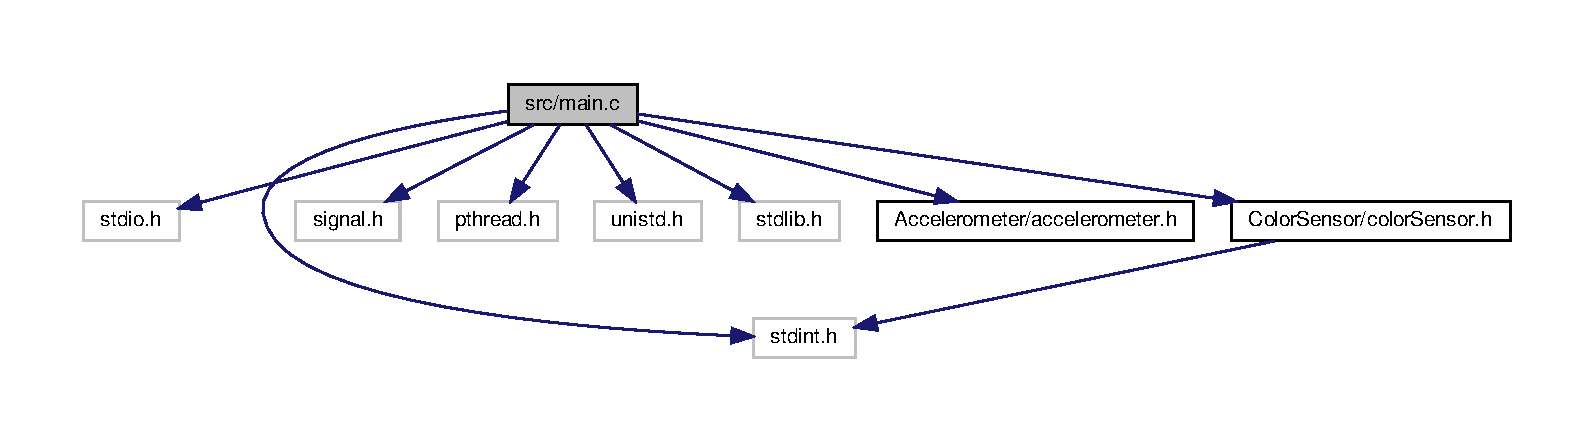
\includegraphics[width=350pt]{main_8c__incl}
\end{center}
\end{figure}
\subsection*{Functions}
\begin{DoxyCompactItemize}
\item 
void \hyperlink{main_8c_aa418b4e82e713f09e062f7c98681ca0b}{sigint\+\_\+isr} (int signal)
\begin{DoxyCompactList}\small\item\em I\+SR for the S\+I\+G\+I\+NT signal. Sets the stop flag to 1 and notifies all sleeping threads. \end{DoxyCompactList}\item 
void $\ast$ \hyperlink{main_8c_afcaf8fe023c53655944cf8fdc667a565}{acc\+\_\+thread\+\_\+fn} (void $\ast$ptr)
\begin{DoxyCompactList}\small\item\em Thread for the acceleration sensor. Starts the sensor and periodically polls its content. When the stop flag is set, closes the sensor. \end{DoxyCompactList}\item 
void $\ast$ \hyperlink{main_8c_a30fede0c10a2e568db2212570e64a274}{color\+\_\+thread\+\_\+fn} (void $\ast$ptr)
\begin{DoxyCompactList}\small\item\em Thread for the color sensor. Starts the sensor and periodically polls its content. When the stop flag is set, closes the sensor. \end{DoxyCompactList}\item 
void $\ast$ \hyperlink{main_8c_a137f0753b4df0eb2e4890cfff561f444}{display\+\_\+thread\+\_\+fn} (void $\ast$ptr)
\begin{DoxyCompactList}\small\item\em Display thread. When there is data ready, prints it to the screen. When the stop flag is set, prints the exit message. \end{DoxyCompactList}\item 
void $\ast$ \hyperlink{main_8c_a58dd83353bca316f6f5d2a03bdf83605}{input\+\_\+thread\+\_\+fn} (void $\ast$ptr)
\begin{DoxyCompactList}\small\item\em Thread to take and process user input. \end{DoxyCompactList}\item 
int \hyperlink{main_8c_ae66f6b31b5ad750f1fe042a706a4e3d4}{main} ()
\begin{DoxyCompactList}\small\item\em Entry point for the project. Starts all the threads and waits for them to finish to close the program. \end{DoxyCompactList}\end{DoxyCompactItemize}


\subsection{Function Documentation}
\mbox{\Hypertarget{main_8c_afcaf8fe023c53655944cf8fdc667a565}\label{main_8c_afcaf8fe023c53655944cf8fdc667a565}} 
\index{main.\+c@{main.\+c}!acc\+\_\+thread\+\_\+fn@{acc\+\_\+thread\+\_\+fn}}
\index{acc\+\_\+thread\+\_\+fn@{acc\+\_\+thread\+\_\+fn}!main.\+c@{main.\+c}}
\subsubsection{\texorpdfstring{acc\+\_\+thread\+\_\+fn()}{acc\_thread\_fn()}}
{\footnotesize\ttfamily void$\ast$ acc\+\_\+thread\+\_\+fn (\begin{DoxyParamCaption}\item[{void $\ast$}]{ptr }\end{DoxyParamCaption})}



Thread for the acceleration sensor. Starts the sensor and periodically polls its content. When the stop flag is set, closes the sensor. 


\begin{DoxyParams}{Parameters}
{\em ptr} & Not used \\
\hline
\end{DoxyParams}
\begin{DoxyReturn}{Returns}
(void$\ast$) Not used 
\end{DoxyReturn}
\mbox{\Hypertarget{main_8c_a30fede0c10a2e568db2212570e64a274}\label{main_8c_a30fede0c10a2e568db2212570e64a274}} 
\index{main.\+c@{main.\+c}!color\+\_\+thread\+\_\+fn@{color\+\_\+thread\+\_\+fn}}
\index{color\+\_\+thread\+\_\+fn@{color\+\_\+thread\+\_\+fn}!main.\+c@{main.\+c}}
\subsubsection{\texorpdfstring{color\+\_\+thread\+\_\+fn()}{color\_thread\_fn()}}
{\footnotesize\ttfamily void$\ast$ color\+\_\+thread\+\_\+fn (\begin{DoxyParamCaption}\item[{void $\ast$}]{ptr }\end{DoxyParamCaption})}



Thread for the color sensor. Starts the sensor and periodically polls its content. When the stop flag is set, closes the sensor. 


\begin{DoxyParams}{Parameters}
{\em ptr} & Not used \\
\hline
\end{DoxyParams}
\begin{DoxyReturn}{Returns}
(void$\ast$) Not used 
\end{DoxyReturn}
\mbox{\Hypertarget{main_8c_a137f0753b4df0eb2e4890cfff561f444}\label{main_8c_a137f0753b4df0eb2e4890cfff561f444}} 
\index{main.\+c@{main.\+c}!display\+\_\+thread\+\_\+fn@{display\+\_\+thread\+\_\+fn}}
\index{display\+\_\+thread\+\_\+fn@{display\+\_\+thread\+\_\+fn}!main.\+c@{main.\+c}}
\subsubsection{\texorpdfstring{display\+\_\+thread\+\_\+fn()}{display\_thread\_fn()}}
{\footnotesize\ttfamily void$\ast$ display\+\_\+thread\+\_\+fn (\begin{DoxyParamCaption}\item[{void $\ast$}]{ptr }\end{DoxyParamCaption})}



Display thread. When there is data ready, prints it to the screen. When the stop flag is set, prints the exit message. 


\begin{DoxyParams}{Parameters}
{\em ptr} & Not used \\
\hline
\end{DoxyParams}
\begin{DoxyReturn}{Returns}
(void$\ast$) Not used 
\end{DoxyReturn}
\mbox{\Hypertarget{main_8c_a58dd83353bca316f6f5d2a03bdf83605}\label{main_8c_a58dd83353bca316f6f5d2a03bdf83605}} 
\index{main.\+c@{main.\+c}!input\+\_\+thread\+\_\+fn@{input\+\_\+thread\+\_\+fn}}
\index{input\+\_\+thread\+\_\+fn@{input\+\_\+thread\+\_\+fn}!main.\+c@{main.\+c}}
\subsubsection{\texorpdfstring{input\+\_\+thread\+\_\+fn()}{input\_thread\_fn()}}
{\footnotesize\ttfamily void$\ast$ input\+\_\+thread\+\_\+fn (\begin{DoxyParamCaption}\item[{void $\ast$}]{ptr }\end{DoxyParamCaption})}



Thread to take and process user input. 


\begin{DoxyParams}{Parameters}
{\em ptr} & Not used \\
\hline
\end{DoxyParams}
\begin{DoxyReturn}{Returns}
(void$\ast$) Not used 
\end{DoxyReturn}
\mbox{\Hypertarget{main_8c_ae66f6b31b5ad750f1fe042a706a4e3d4}\label{main_8c_ae66f6b31b5ad750f1fe042a706a4e3d4}} 
\index{main.\+c@{main.\+c}!main@{main}}
\index{main@{main}!main.\+c@{main.\+c}}
\subsubsection{\texorpdfstring{main()}{main()}}
{\footnotesize\ttfamily int main (\begin{DoxyParamCaption}{ }\end{DoxyParamCaption})}



Entry point for the project. Starts all the threads and waits for them to finish to close the program. 

\begin{DoxyReturn}{Returns}
(int) Exit code of the program 
\end{DoxyReturn}
\mbox{\Hypertarget{main_8c_aa418b4e82e713f09e062f7c98681ca0b}\label{main_8c_aa418b4e82e713f09e062f7c98681ca0b}} 
\index{main.\+c@{main.\+c}!sigint\+\_\+isr@{sigint\+\_\+isr}}
\index{sigint\+\_\+isr@{sigint\+\_\+isr}!main.\+c@{main.\+c}}
\subsubsection{\texorpdfstring{sigint\+\_\+isr()}{sigint\_isr()}}
{\footnotesize\ttfamily void sigint\+\_\+isr (\begin{DoxyParamCaption}\item[{int}]{signal }\end{DoxyParamCaption})}



I\+SR for the S\+I\+G\+I\+NT signal. Sets the stop flag to 1 and notifies all sleeping threads. 


\begin{DoxyParams}{Parameters}
{\em signal} & Signal identifier \\
\hline
\end{DoxyParams}

%--- End generated contents ---

% Index
\backmatter
\newpage
\phantomsection
\clearemptydoublepage
\addcontentsline{toc}{chapter}{Index}
\printindex

\end{document}
